%% TEMPO manuscript — INFORMS Transportation Science submission template
%% Build: pdflatex main && bibtex main && pdflatex main && pdflatex main

\documentclass[trsc,sglanonrev]{informs4}
\usepackage{eqndefns-left}
\RequirePackage{tgtermes}
\RequirePackage{mathptmx}
\RequirePackage{bm}
\RequirePackage{endnotes}
\usepackage{booktabs}
\usepackage{graphicx}

\OneAndAHalfSpacedXII

\usepackage{algorithm}
\usepackage{algpseudocode}

\usepackage{natbib}
 \bibpunct[, ]{(}{)}{,}{a}{}{,}%
 \def\bibfont{\small}%
 \def\bibsep{\smallskipamount}%
 \def\bibhang{24pt}%
 \def\newblock{\ }%
 \def\BIBand{and}%

\EquationsNumberedThrough
\TheoremsNumberedThrough
\ECRepeatTheorems

\MANUSCRIPTNO{TRSC-0000-2026.00}

% ── notation shortcuts ───────────────────────────────────────────────
\newcommand{\E}{\mathbb{E}}
\newcommand{\Prob}{\mathbb{P}}
\newcommand{\N}{\mathcal{N}}
\newcommand{\F}{\mathcal{F}}
\newcommand{\KL}{\mathrm{KL}}
\newcommand{\Rmax}{\mathrm{R}}

\begin{document}

\RUNAUTHOR{Dang, Vu, and Nguyen}

\RUNTITLE{When to Replan in Stochastic Vehicle Routing}

\TITLE{When to Replan: A Decision-Relevant E-Process for Anytime-Valid
Re-Optimization in Stochastic Vehicle Routing}

\ARTICLEAUTHORS{%
\AUTHOR{Quang-Vinh Dang}
\AFF{Department of Logistics, British University Vietnam, Hung Yen,
Vietnam, \EMAIL{vinh.dq4@buv.edu.vn}}
\AUTHOR{Hoang-Viet Vu}
\AFF{Department of Logistics, British University Vietnam, Hung Yen,
Vietnam, \EMAIL{30066555@st.buv.edu.vn}}
\AUTHOR{Phuc-Son Nguyen}
\AFF{UEH University, Ho Chi Minh City, Vietnam,
\EMAIL{sonnp.3393@ueh.edu.vn}}
}

\ABSTRACT{%
A dispatcher who has committed a fleet to routes optimized against a
planning model faces a question that recurs every minute of the
operating day: has enough gone wrong to justify the cost and
disruption of re-optimizing, or is the plan still worth following? We
formalize this question as a sequential hypothesis test, run
continuously, of the null hypothesis that the day is unfolding
according to the planning model's joint law over travel time, demand,
dwell time, accidents, and vehicle breakdowns. The test statistic is an
e-process --- a nonnegative process whose expectation under the null
never exceeds one --- built as a running product of per-factor
likelihood-ratio bets; Ville's inequality then bounds the probability
of a false alarm uniformly over the entire monitoring horizon, so the
dispatcher may inspect the statistic after every event without
inflating the error rate, a guarantee no fixed-checkpoint or
fixed-threshold monitor provides. Our contribution is to couple the
design of these bets to the economics of the routing plan itself: each
factor's statistical evidence is weighted, at every instant, by a
predictable sensitivity computed from the plan's own fitted
continuation costs, so that the monitor spends its power exactly where
a small deviation would flip the optimal recourse decision, and we
prove this coupling remains a valid e-process and is, moreover,
growth-optimal against the class of cost-relevant alternatives. Four
new results connect the statistical trigger to routing economics: a
regret bound for the induced re-optimization policy, a closed-form
expression for the significance level a dispatcher should use as a
function of fleet economics rather than statistical convention, a
theorem showing that waiting for evidence dominates replanning
immediately once uncertainty is realized, and the growth-optimality
result above. We validate the resulting monitor, TEMPO, across 73
synthetic instances spanning established vehicle-routing benchmarks and
real road networks, a 19-scenario stochastic-drift grid, a pilot on
real last-mile delivery data, and head-to-head comparisons against ten
baselines spanning classical sequential tests, a 2024 nonparametric
e-detector framework, a 2026 chance-constrained model-predictive
strategy, and a 2025 reinforcement-learning policy for time-dependent
stochastic routing. At matched false-alarm budgets the coupled monitor
detects harmful drift faster and more often than every baseline on
nearly every scenario, and a companion experiment on re-optimization
cost shows that waiting for its alarm, rather than replanning at the
first sign of trouble, lowers realized fleet cost by a further six
percentage points.
}%

\KEYWORDS{vehicle routing, sequential change detection, e-values,
anytime-valid inference, dynamic re-optimization, stochastic
programming}

\maketitle

% ══════════════════════════════════════════════════════════════════
\section{Introduction}\label{sec:intro}

Every dispatcher who operates a fleet under a routing plan faces the
same recurring decision, and it is not the decision that the vehicle
routing literature usually studies. The plan itself --- which customer
each vehicle visits, and in what order --- is typically the output of
a careful optimization against a model of travel times, demand, and
service times. Once the fleet is on the road, that model is tested
continuously against reality: a road runs slower than forecast, a
customer's parcel is heavier than its historical average, a delivery
takes longer to sign for, an accident closes a lane, a vehicle breaks
down. None of these events individually justifies tearing up the plan
and re-solving the routing problem from the vehicles' current
positions --- re-optimization is neither free nor riskless, since it
consumes computation, disrupts drivers who have already committed to a
sequence, and can occasionally make things worse if it acts on noise
rather than signal. Yet delaying re-optimization has its own cost: a
plan that no longer matches the world accumulates late deliveries,
capacity breaches, and unnecessary distance with every additional
event it is allowed to govern. The operational question, then, is not
only \emph{how} to re-optimize but \emph{when}, and it is this second
question that the present paper answers.

Two families of answers exist in practice, and both are unsatisfying
on close inspection. The first is periodic: re-solve the routing
problem every $\Delta$ minutes or every $\Delta$ completed stops,
regardless of whether anything has actually gone wrong
\citep{pillac2013review}. Periodic and rolling-horizon re-optimization
is the industrial default, and recent work continues to refine the
re-solve itself --- for instance as a chance-constrained model
predictive control problem \citep{he2026smpc} --- without revisiting
the question of when the re-solve should happen; the schedule is
exogenous to the data. The second family is reactive but ad hoc: replan
once cumulative lateness exceeds a tuned threshold, or once a load
gets ``too close'' to capacity. Thresholds tuned this way have no
error-rate guarantee, invite alarm fatigue when set too tight, and miss
slow, compounding drift when set too loose. A third possibility,
familiar from the statistics of sequential monitoring, is to treat the
question honestly as a hypothesis test: classical sequential
detectors such as CUSUM \citep{page1954} and its data-stream
descendants \citep{gama2014survey} are designed exactly for ``has the
data-generating process changed,'' and in principle a dispatcher could
run one per uncertainty factor and replan on the first alarm. The
difficulty is that classical sequential tests control their false-alarm
rate only at a threshold calibrated to the specific monitoring horizon
and null distribution; used off the shelf, with the textbook constant
or a threshold copied from a different operating regime, their realized
false-alarm rate can exceed the nominal level by a wide margin, exactly
because the guarantee is not anytime-valid --- it does not survive the
dispatcher looking whenever she likes. Bayesian online change-point
detection \citep{adams2007bayesian} sidesteps threshold tuning with a
posterior probability of a regime change, but at the cost of any
frequentist error-rate control at all.

A separate and more recent strand of statistics offers exactly the
property routing dispatch needs: \emph{anytime-valid} sequential
testing built on e-values and e-processes
\citep{shafer2021testing,ramdas2023safi}. An e-process is a
nonnegative stochastic process whose expectation never exceeds one
under the null hypothesis; by Ville's maximal inequality, the
probability that it ever crosses a threshold $1/\alpha$, over an
arbitrarily long and even data-dependent monitoring horizon, is at
most $\alpha$. A dispatcher can therefore watch the process after every
single event --- every leg traversed, every stop serviced --- and
replan the instant it crosses the threshold, with a false-alarm
guarantee that holds regardless of how often she looks or how she
decides to stop looking. This machinery is not new; it is the modern
form of Wald's sequential probability ratio test, understood through
the lens of testing by betting, and a 2024 line of work already
generalizes it to nonparametric change detection through the
\emph{e-detector} framework \citep{shin2024edetectors}. What is new in
this paper is not the statistical technology but its coupling to the
economics of the routing problem it monitors. A generic e-process,
built from statistically natural bets on each uncertainty factor,
spends its statistical power uniformly: it is exactly as alert to a
demand fluctuation that would never come close to breaching a
vehicle's capacity as to one that would. This is wasteful, because the
routing plan itself already encodes, through its fitted continuation
costs and per-stop recourse prices, exactly where a small perturbation
would flip the optimal decision and where it would not. Our companion
paper on the planning and recourse layer \citep{dang2026baton} builds
those continuation costs as a backward-induction value function over
the demand process; the present paper shows how to read that value
function's local sensitivity back into the design of a monitoring
statistic, so that the same fitted model that tells the fleet
\emph{what} to do when capacity is breached also tells the monitor
\emph{where to look}.

We call the resulting monitor TEMPO --- a Tilted E-Martingale Process
for Online re-optimization --- and its four contributions are as
follows.

First, we construct a master e-process over five coupled uncertainty
factors --- travel time (diurnal, weather-modulated, and
congestion-shocked), demand, dwell time, zone-wide accidents, and
vehicle breakdowns --- each contributing a likelihood-ratio bet whose
tilt is scaled, at every event, by a \emph{predictable sensitivity}
computed from the plan's own fitted economics: how close the running
load sits to its capacity-breach boundary, how much of the remaining
route lies inside an affected zone, how much schedule slack remains.
Because these sensitivities are measurable with respect to the
information available strictly before the event they weight, the
tilted process remains a valid e-process with exactly the same
anytime-valid guarantee as the untilted one --- the coupling is free of
statistical cost.

Second, we prove four theorems that are new to the routing literature
even though the statistical machinery underneath them is not: a
cost-regret bound for the re-optimization policy the monitor induces
(Theorem~\ref{thm:regret}); a closed-form expression, derived from that
bound, for the significance level a dispatcher should adopt as a ratio
of fleet economics rather than a statistical convention
(Corollary~\ref{cor:alphastar}); a theorem formalizing why waiting for
evidence before rebalancing a fleet's remaining capacity dominates
rebalancing at the first sign of trouble
(Theorem~\ref{thm:waiting}); and a growth-optimality theorem showing
that the sensitivity-tilted bet is, among all predictable betting
strategies with the same statistical budget, the one that minimizes
detection delay against the class of alternatives that actually matter
to the routing cost (Theorem~\ref{thm:growth}).

Third, we separate the question of \emph{when} to replan from the
question of \emph{what} the new plan should be: the trigger is
paired with a pluggable family of mid-route replanners, from
single-vehicle re-sequencing to fleet-wide rebalancing, so that the
statistical layer of the paper composes with any re-optimization
routine a fleet already uses.

Fourth, we validate TEMPO on a scale unusual for this literature: 73
synthetic instances spanning two established vehicle-routing
benchmarks and nineteen real road networks, a grid of 19 stochastic
drift scenarios crossing five uncertainty factors with null,
mild-to-severe, ramped, transient, and compound variants, a pilot on
fifty real last-mile routes from the 2021 Amazon Last-Mile Routing
Research Challenge \citep{merchan2024amazon}, and head-to-head
comparisons against ten baselines including two 2024
e-detector variants \citep{shin2024edetectors}, the periodic-re-solve
cadence of a 2026 chance-constrained strategy \citep{he2026smpc}, and
the rolling-horizon foil against which a 2025 deep-reinforcement-
learning policy for time-dependent stochastic routing was itself
benchmarked \citep{chen2025dgta}. At a matched false-alarm budget the
coupled monitor dominates or ties every baseline on nearly every
scenario in the grid, and a companion cost experiment confirms
Theorem~\ref{thm:waiting} directly: triggering a fleet-wide rebalance
on the monitor's alarm, rather than at the first stop after a
suspected drift, lowers realized day cost by a further six percentage
points because the rebalancer acts on realized loads rather than
priors.

The remainder of the paper is organized as follows.
Section~\ref{sec:related} positions the paper against dynamic vehicle
routing, classical sequential change detection, and the anytime-valid
inference literature. Section~\ref{sec:model} formalizes the
multi-factor stochastic routing day and its null hypothesis.
Section~\ref{sec:eprocess} builds the master e-process and proves its
validity. Section~\ref{sec:coupling} introduces the decision-relevant
predictable tilts that couple the monitor to the plan's economics.
Section~\ref{sec:tempo} assembles TEMPO's adaptive betting, dual-regime
combination, and rare-event separation into the final monitor.
Section~\ref{sec:theory} proves the four economic theorems.
Section~\ref{sec:decision} describes the pluggable replanning layer.
Section~\ref{sec:study} reports the computational study.
Section~\ref{sec:discussion} discusses managerial implications, and
Section~\ref{sec:conclusion} concludes.

% ══════════════════════════════════════════════════════════════════
\section{Related work}\label{sec:related}

\textbf{Dynamic and stochastic vehicle routing.} The question of
re-optimizing a routing plan as information arrives is as old as the
dynamic vehicle routing literature itself; \citet{pillac2013review}
survey the dominant re-optimization architectures, nearly all of which
re-solve on an exogenous clock --- every $\Delta$ minutes, every
completed stop, or at pre-committed decision epochs --- rather than in
response to accumulated statistical evidence. \citet{he2026smpc}
develop a chance-constrained model predictive control strategy for
vehicle routing with correlated stochastic service times whose
re-solve cadence is exactly this periodic pattern; our periodic
baseline reproduces its trigger mechanism directly, since the
time-window MILP it re-solves is outside the scope of the present
paper's harness. \citet{chen2025dgta} take a different route entirely,
training a Dynamic Graph Temporal Attention reinforcement-learning
policy that reacts to time-dependent stochastic travel times
end-to-end, with no explicit change-detection layer and consequently no
error-rate guarantee of any kind; their own baseline for that policy is
the rolling-horizon heuristic of \citet{gmira2021rollingopt}, which we
also reproduce. None of this literature poses re-optimization timing as
a calibrated statistical decision, which is precisely the gap the
present paper fills.

\textbf{Classical sequential change detection.} The CUSUM statistic of
\citet{page1954} and its many descendants, surveyed for the data-stream
setting by \citet{gama2014survey}, remain the workhorse tools for
deciding when a stochastic process has drifted. Both require a
threshold $h$ calibrated to the specific null distribution and
monitoring horizon; used with a textbook or borrowed constant, their
realized false-alarm probability need not equal, or even bound, the
nominal level, because the guarantee CUSUM actually enjoys is an
average-run-length bound under continuous, unbounded operation rather
than a probability bound over a bounded, data-dependent stopping time.
\citet{adams2007bayesian} replace the frequentist threshold with a
posterior probability of a regime change under a Bayesian online
change-point model, trading the calibration problem for the absence of
any frequentist type-I error control. Section~\ref{sec:study} shows
this distinction is not a technicality: oracle-calibrating CUSUM and
its Page--Hinkley relative to match TEMPO's realized false-alarm rate,
exactly the generous comparison this literature invites, still leaves
both classical detectors behind on most of the 19-scenario grid.

\textbf{Anytime-valid inference and e-processes.} A test martingale, or
e-process, is a nonnegative supermartingale under the null with
expectation at most one; Ville's inequality
\citep{ville1939etude} bounds the probability that such a process ever
exceeds $1/\alpha$ by $\alpha$, uniformly over an arbitrary, even
adaptively chosen, stopping time. \citet{shafer2021testing} reframes
this classical fact as ``testing by betting'': an e-value is the payoff
of a bet against the null that a rational bettor could have placed
without knowing the outcome, and the game-theoretic perspective unifies
sequential testing, confidence sequences, and multiple testing under
one anytime-valid umbrella, surveyed by \citet{ramdas2023safi}.
\citet{waudbysmithramdas2024} develop adaptive, data-driven betting
strategies (GRAPA and its regularized variant aGRAPA) that learn the
growth-optimal tilt online from past increments while remaining
predictable, and hence valid; TEMPO's adaptive channel bets are a
direct application of this idea. \citet{vovkwang2021combining}
establish that mixtures and simple averages of e-values are themselves
e-values, which licenses both the fixed-grid mixture bets of
Section~\ref{sec:eprocess} and TEMPO's dual-regime combination in
Section~\ref{sec:tempo}. Closest in spirit to the present paper is the
e-detector framework of \citet{shin2024edetectors}, which builds
nonparametric change detectors by restarting an e-process at every
candidate change-point and combining the restarted copies by a running
sum (Shiryaev--Roberts) or running maximum (CUSUM-like) rule; we
implement both variants using exactly TEMPO's own per-factor bets, with
the cost-relevance tilt switched off, as a controlled ablation that
isolates general nonparametric restart machinery from TEMPO's specific
coupling to routing economics (Section~\ref{sec:study}). We are careful
to distinguish the e-detector's native guarantee --- an average-run-
length bound over an indefinitely long stream (their Theorem 2.4) ---
from the finite-window false-alarm probability bound TEMPO's own Ville
argument delivers; the two are not interchangeable, and conflating them
is a mistake the reproduction in Section~\ref{sec:study} corrects
through matched oracle calibration.

None of this statistical literature, to our knowledge, couples the
design of the betting strategy to the economics of a decision the
statistic will trigger. The present paper's contribution is exactly
that coupling, made precise in Sections~\ref{sec:coupling}
and~\ref{sec:theory}: the plan's own fitted continuation costs, the
central object of \citet{dang2026baton}'s optimal-stopping recourse
policy, supply the predictable sensitivity that tells each channel's
bet how hard to push, and Theorem~\ref{thm:growth} shows this choice is
not merely intuitive but growth-optimal against the class of
alternatives that actually move the routing cost.

% ══════════════════════════════════════════════════════════════════
\section{The stochastic routing day}\label{sec:model}

We take as given a routing plan --- a sequence of stops per vehicle ---
produced by any planning-time optimizer against a demand and travel-
time model; in our computational study this plan is produced by the
adaptive large neighborhood search of \citet{dang2026baton}, but
nothing in the construction below depends on how the plan was built.
The paper's object of study is what happens \emph{after} the plan is
fixed and the fleet departs: a chronological stream of events, each an
independent opportunity to ask whether the plan is still trustworthy.

\subsection{Events and the null hypothesis}

Fix one vehicle's route, indexed by stop $k = 1, \dots, m$. The
execution of the route generates, in chronological order, an event for
each of five factors at each stop or leg: the travel time on the leg
into stop $k$, the number of zone-wide accidents observed while
traversing that leg, an indicator of whether the vehicle breaks down on
that leg, the net demand realized at stop $k$, and the dwell time spent
servicing it. We index the resulting event stream by $n = 1, \dots,
N$, $N = 5m$, and write $\F_{n-1}$ for the $\sigma$-algebra generated by
everything realized strictly before event $n$ --- the vehicle's clock
time, its running net load, the remaining route, and every earlier
realization. All quantities defined ``before'' event $n$ below are by
construction $\F_{n-1}$-measurable; this predictability is the single
technical fact on which every validity result in the paper rests.

The planning model specifies a null law $P_0$ for each factor,
conditional on a small number of exogenous covariates that the monitor
is allowed to see \emph{without} penalty --- the whole point of writing
these laws explicitly is to make sure that a deviation the plan already
anticipated is never mistaken for evidence against it.

\emph{Travel time.} The travel time on the leg into stop $k$, departing
at clock time $t$, is
\begin{align}
T_k &= \tau_k \, m(t) \, w(R) \, \exp(\varepsilon_k), \label{eq:travel}\\
\varepsilon_k &\sim \N\!\left(-\tfrac{1}{2}\sigma_T^2, \sigma_T^2\right),
\notag
\end{align}
where $\tau_k$ is the free-flow leg time, $m(\cdot)$ is a known diurnal
multiplier curve (morning and evening peaks), $R \in \{0,1\}$ is an
exogenous rain indicator realized once per day with known probability
and known multiplier $w(1) = w_{\mathrm{rain}} > 1 = w(0)$, and the mean
of $\varepsilon_k$ is chosen so that $\E[\exp(\varepsilon_k)] = 1$: the
multiplicative noise is mean-preserving. Both $m(t)$ and $R$ are
covariates of the conditional null, not targets of the test --- a traffic
jam at the evening peak that the diurnal curve already predicted, or a
day that a forecast correctly called rainy, produces \emph{no} evidence
against $P_0$ under this construction, precisely because the monitor
conditions on them.

\emph{Demand.} The net demand increment at stop $k$ (pickup volume
minus delivery volume, in the simultaneous pickup-and-delivery setting
of \citet{dang2026baton}) is
\begin{equation}\label{eq:demand}
g_k \sim \N(\mu_k, \sigma_{g,k}^2),
\end{equation}
with $(\mu_k, \sigma_{g,k})$ the planning model's stop-level mean and
standard deviation, fitted from the same historical demand scenarios
used to build the route.

\emph{Dwell time.} The service time at stop $k$ depends on the realized
demand magnitude,
\begin{align}
S_k &= a + b\,|g_k| + \eta_k, \qquad S_k \ge 0, \label{eq:dwell}\\
\eta_k &\sim \N(0, \sigma_S^2), \notag
\end{align}
with $(a,b,\sigma_S)$ fitted service-time parameters.

\emph{Accidents.} Zone-wide accidents are observed as a Poisson process
of rate $\lambda_0$ per hour under $P_0$; the count observed while
traversing a leg of realized duration $T_k$ is
\begin{equation}\label{eq:accident}
n_k \sim \mathrm{Poisson}(\lambda_0 T_k).
\end{equation}

\emph{Breakdowns.} Each leg carries an independent breakdown indicator
\begin{equation}\label{eq:breakdown}
x_k \sim \mathrm{Bernoulli}(p_0), \qquad p_0 \text{ small}.
\end{equation}

\subsection{Change-point drift}

A day is either on-model, generated entirely from the laws above, or it
drifts: at an (unknown to the monitor) clock time $t^\ast$, one or more
factors switch to an alternative law $P_1$. We parameterize drift by a
kind (which factor), a magnitude, an onset time $t^\ast$, and a profile
--- a step onset, a ramp reaching full intensity over a fixed window, or
a transient episode that clears after a fixed duration --- together
with, for the travel-time factor specifically, a spatial extent: a
congestion pocket centered at a point in the service area whose radius
grows after $t^\ast$, so that only legs whose destination currently
lies inside the pocket are slowed. This last extension matters for a
fleet: it gives drift a \emph{where} as well as a \emph{when}, so that
vehicles routed far from the affected zone correctly contribute
on-model evidence even while the day, taken as a whole, has drifted.
Table~\ref{tab:scenarios} in Section~\ref{sec:study} catalogs the
resulting 19-scenario grid used throughout the computational study.

Under drift, each factor's law shifts multiplicatively in its natural
parameter: the travel-time log-mean in Equation~\eqref{eq:travel}
shifts by $\rho(t)\log(\text{magnitude})$, the demand mean in
Equation~\eqref{eq:demand} shifts by $\rho(t)\times\text{magnitude}
\times\sigma_{g,k}$, the dwell mean in Equation~\eqref{eq:dwell}
analogously, the accident rate in Equation~\eqref{eq:accident} is
scaled by a multiplicative factor, and the breakdown probability in
Equation~\eqref{eq:breakdown} likewise, where $\rho(t) \in [0,1]$ is the
drift's intensity profile (zero before $t^\ast$, one under a step
profile, linearly ramping under a ramp profile, and returning to zero
after a transient clears). No structural assumption of the paper
requires drift to be present or of any particular size; Section
\ref{sec:theory} states its regret bound for a general per-event
Kullback--Leibler separation $\KL(P_1\Vert P_0) \ge \KL_{\min} > 0$
between the post-change law and the null.

% ══════════════════════════════════════════════════════════════════
\section{The master e-process}\label{sec:eprocess}

We now build a single statistic that tests, continuously, whether the
event stream of Section~\ref{sec:model} is following $P_0$.

\subsection{E-values and e-processes}

\begin{definition}\label{def:evalue}
A random variable $e \ge 0$ measurable with respect to $\F_n$ is an
\emph{e-value} for testing $P_0$ at event $n$ if
$\E_{P_0}[e \mid \F_{n-1}] \le 1$. A process $(E_n)_{n \ge 0}$ with
$E_0 = 1$ is an \emph{e-process} if $E_n = E_{n-1} \cdot e_n$ for a
sequence of e-values $e_n$; equivalently, $(E_n)$ is a nonnegative
supermartingale under $P_0$ with $\E_{P_0}[E_n] \le 1$ for every $n$.
\end{definition}

\begin{lemma}[Ville's inequality; \citealp{ville1939etude}]\label{lem:ville}
If $(E_n)$ is a nonnegative supermartingale with $E_0 = 1$, then for
every $\alpha \in (0,1)$,
\begin{equation}\label{eq:ville}
\Prob_{P_0}\Bigl(\sup_{n \ge 0} E_n \ge \tfrac{1}{\alpha}\Bigr) \le \alpha.
\end{equation}
\end{lemma}

Lemma~\ref{lem:ville} is the entire source of the anytime-valid
guarantee this paper relies on: the supremum on the left is taken over
\emph{all} $n$, including a data-dependent stopping rule chosen by the
dispatcher after seeing the data, so a monitor built from an e-process
may be inspected after every single event without the false-alarm
probability exceeding $\alpha$. No analogous statement holds for a
statistic calibrated only at pre-committed checkpoints, which is
exactly the distinction Section~\ref{sec:study} exploits in the
Bonferroni-fixed baseline.

\subsection{Per-channel bets}

Each factor of Section~\ref{sec:model} contributes a bet at the event
where it is realized; the four continuous and count factors are
exponential-family mean-shift likelihood-ratio statistics, and the
breakdown factor is a rare-event stake. Write $z_n = (g_n - \mu_n)/
\sigma_{g,n}$, $(\log T_n - \mu_{\log T,n})/\sigma_T$, or
$(S_n - \mu_{S,n})/\sigma_S$ for the standardized residual of whichever
continuous factor is realized at event $n$, so that $z_n \sim \N(0,1)$
under $P_0$ by Equations~\eqref{eq:travel}--\eqref{eq:dwell}. For a
tilt $\theta \in \mathbb{R}$,
\begin{equation}\label{eq:gaussianbet}
e^{\mathrm{g}}(\theta; z_n) = \exp\!\left(\theta z_n - \tfrac{1}{2}\theta^2\right)
\end{equation}
satisfies $\E_{P_0}[e^{\mathrm{g}}(\theta; z_n) \mid \F_{n-1}] = 1$ for
any $\F_{n-1}$-measurable $\theta$, since $z_n \mid \F_{n-1} \sim
\N(0,1)$ under $P_0$ and Equation~\eqref{eq:gaussianbet} is exactly the
$\N(\theta,1)$-versus-$\N(0,1)$ likelihood ratio evaluated at $z_n$.
For the accident count $n_k$ with conditional mean $\lambda_0 T_k$
under $P_0$,
\begin{equation}\label{eq:poissonbet}
e^{\mathrm{p}}(\theta; n_k, \lambda_0 T_k) = \exp\!\bigl(\theta n_k -
\lambda_0 T_k (e^\theta - 1)\bigr)
\end{equation}
is the Poisson tilted likelihood ratio, again conditional mean one for
any predictable $\theta$. For the breakdown indicator $x_k$ with
$\E_{P_0}[x_k] = p_0$, a stake $w \in [0,1]$ gives the rare-event bet
\begin{equation}\label{eq:bernoullibet}
e^{\mathrm{b}}(w; x_k, p_0) = 1 - w + w\,\frac{x_k}{p_0},
\end{equation}
which has conditional mean $1 - w + w\,p_0/p_0 = 1$ for any
predictable $w$, and is chosen small enough that a quiet leg costs only
$\log(1-w) \approx -w$ in log-wealth while a single breakdown, being
$\gg 1/p_0$ times its null probability, crosses any reasonable alarm
threshold on its own --- a hard, near-point-mass event needs no further
statistical refinement to be detected instantly.

Robustness to an unknown tilt magnitude is bought, at zero cost to
validity, by mixing over a fixed grid $\Theta = \{\theta_1, \dots,
\theta_J\}$ with weights $\pi_j \ge 0$, $\sum_j \pi_j = 1$:
\begin{equation}\label{eq:mixture}
e(z_n) = \sum_{j=1}^J \pi_j\, e^{\mathrm{g}}(\theta_j; z_n).
\end{equation}

\begin{lemma}[mixtures of e-values are e-values; \citealp{vovkwang2021combining}]\label{lem:mixture}
If $e^{(1)}, \dots, e^{(J)}$ are e-values for the same null with
respect to $\F_{n-1}$, then any convex combination
$\sum_j \pi_j e^{(j)}$ with predictable, nonnegative $\pi_j$ summing to
one is also an e-value.
\end{lemma}

Lemma~\ref{lem:mixture} follows immediately from the linearity of
conditional expectation and Definition~\ref{def:evalue}; it licenses
both the fixed-grid mixture of Equation~\eqref{eq:mixture} and the
dual-regime combination of Section~\ref{sec:tempo}.

\subsection{The master process and Proposition~\ref{prop:validity}}

At each event $n$ exactly one factor is realized; write $e_n$ for that
factor's mixture bet, evaluated at $z_n$, $n_k$, or $x_k$ as
appropriate. The master e-process is the running product
\begin{equation}\label{eq:master}
E_n = \prod_{i=1}^n e_i,
\end{equation}
and the monitor alarms at
\begin{equation}\label{eq:alarm}
\tau = \inf\{n : E_n \ge 1/\alpha\}.
\end{equation}

\begin{proposition}[validity of the master process]\label{prop:validity}
For any choice of predictable tilts $\theta_j(n)$ (respectively stakes
$w(n)$) taking values in a fixed grid, the process $(E_n)$ of
Equation~\eqref{eq:master} is a nonnegative supermartingale under $P_0$
with $\E_{P_0}[E_n] \le 1$ for every $n$, and consequently
$\Prob_{P_0}(\exists\, n : E_n \ge 1/\alpha) \le \alpha$.
\end{proposition}

\begin{proof}{Proof}
By Lemma~\ref{lem:mixture} each $e_n$ is an e-value with respect to
$\F_{n-1}$ regardless of which factor fires at event $n$, since a
channel that does not fire at $n$ contributes an implicit factor of
one and hence cannot affect the conditional mean. By the tower
property,
\[
\E_{P_0}[E_n \mid \F_{n-1}] = E_{n-1}\, \E_{P_0}[e_n \mid \F_{n-1}] \le
E_{n-1},
\]
so $(E_n)$ is a nonnegative supermartingale with $E_0 = 1$, and
$\E_{P_0}[E_n] \le \E_{P_0}[E_{n-1}] \le \dots \le E_0 = 1$ by
induction. The tail bound is Lemma~\ref{lem:ville} applied to this
process. \Halmos
\end{proof}

The crux of Proposition~\ref{prop:validity}, and the fact that makes
every subsequent refinement of the paper free of statistical cost, is
that the tilt $\theta_j(n)$ or stake $w(n)$ used at event $n$ may
depend on absolutely anything realized strictly before event $n$ ---
including, in particular, a sensitivity computed from the routing
plan's own economics, which is exactly what Section~\ref{sec:coupling}
introduces --- without disturbing the tower-property argument above.
The only requirement is measurability with respect to $\F_{n-1}$; the
tilt may not peek at the very observation it is about to weight.

Figure~\ref{fig:explainer}, panel A, illustrates the resulting process
empirically on sixty simulated null days for one route: every
trajectory stays comfortably below the alarm threshold $1/\alpha$, and
across the full grid of Section~\ref{sec:study} the realized
false-alarm rate never exceeds the nominal $\alpha$, exactly as
Proposition~\ref{prop:validity} predicts.

\begin{figure}
\FIGURE
{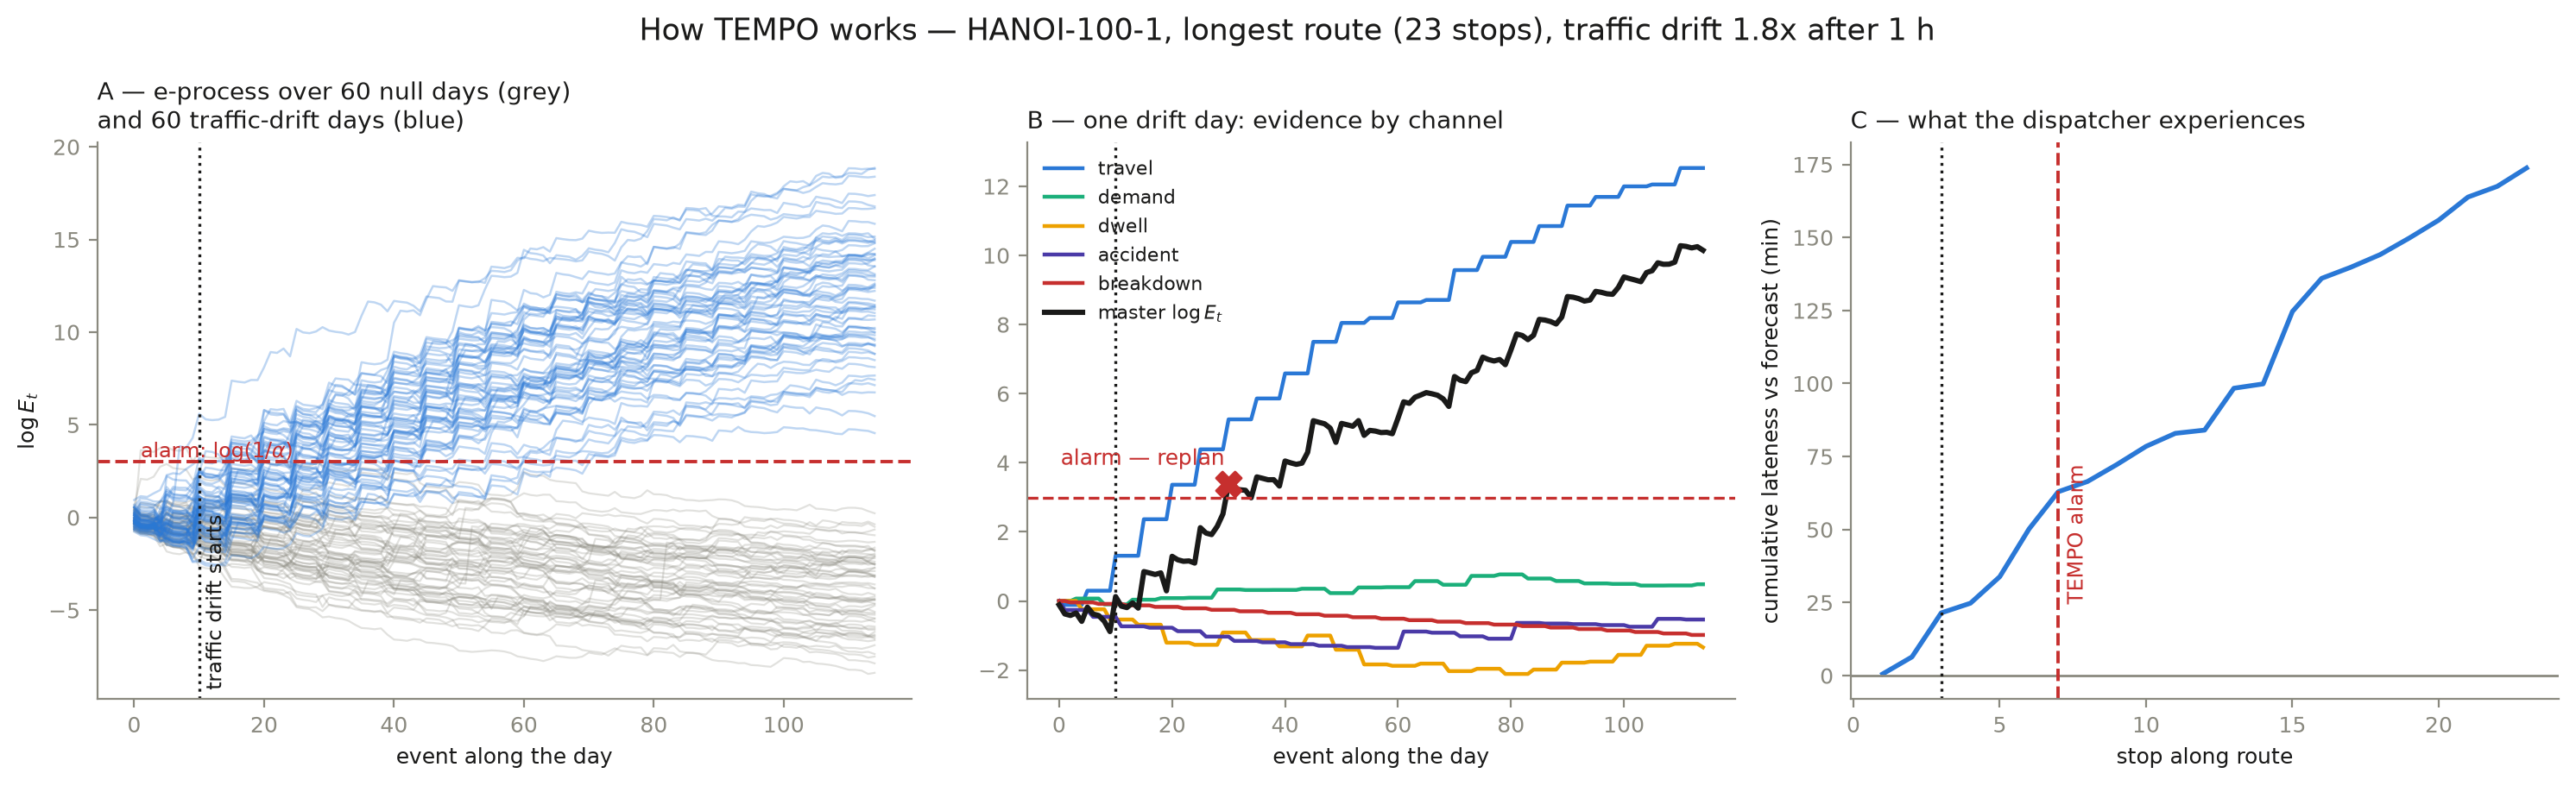
\includegraphics[width=\textwidth]{figures/tempo_fig1_explainer.png}}
{How the master e-process behaves on-model and under drift.
\label{fig:explainer}}
{Panel A: the log e-process over sixty simulated null days for one
route (grey), all remaining below the alarm threshold. Panel B: the
per-channel log-evidence decomposition of Equation~\eqref{eq:master}
on a single drift day, showing which factor drives the alarm. Panel C:
the resulting alarm time translated into the dispatcher's view of the
day.}
\end{figure}

% ══════════════════════════════════════════════════════════════════
\section{Decision-relevant predictable tilts}\label{sec:coupling}

A master process built from Equation~\eqref{eq:mixture} alone is
statistically sound but economically indiscriminate: it is exactly as
alert to a demand fluctuation that leaves a vehicle's residual capacity
untouched as to one that pushes it to the brink of a breach, and
exactly as alert to a jam on a leg the vehicle will never traverse as
to one directly ahead of it. This section couples the tilt itself to
the routing plan's own economics, so that the monitor's statistical
power is spent where a deviation would actually change the optimal
recourse decision.

\subsection{Sensitivity as a predictable weight}

For each factor $k \in \{\text{travel}, \text{demand}, \text{dwell},
\text{accident}, \text{breakdown}\}$ we define a \emph{sensitivity}
$s_k(n) \in [0,1]$, computed entirely from information available at
$\F_{n-1}$, that measures how decision-relevant a unit of drift in
factor $k$ would be at event $n$ given the plan's current state. The
tilt actually applied at event $n$ is then $\theta_j(n) = \theta_j
\cdot s_k(n)$ for each grid point $\theta_j$ --- the grid itself is
unchanged, but its reach is scaled by the plan's own sensitivity.

\emph{Demand.} \citet{dang2026baton}'s recourse policy intervenes on a
route exactly when the fitted continuation cost of carrying the
current load onward, $\widehat C(W)$, exceeds the cheapest available
recourse price, $\min(H, R+F)$ for a handoff price $H$ and a
restock-then-continue price $R+F$; the optimal-stopping boundary is
therefore a level set of the running load $W$ relative to the route's
residual capacity $B$. We define
\begin{equation}\label{eq:sensdemand}
s_{\mathrm{demand}}(n) = 1 - \min\!\left(\frac{|B - W_{n-1}|}{B}, 1\right),
\end{equation}
the closeness of the running load $W_{n-1}$, before event $n$'s demand
realizes, to the capacity boundary $B$: near the boundary, a small
demand shock is enough to flip the optimal recourse decision, and the
sensitivity is large; early in the route, with $W_{n-1}$ far from $B$,
the same shock changes nothing, and the sensitivity --- correctly ---
is small.

\emph{Travel, dwell, and accidents.} These three factors' decision
relevance is governed by how much of the plan remains to be executed,
since a leg-time or dwell-time shock early in a long remaining route
compounds over more downstream stops than the same shock late in a
short one:
\begin{equation}\label{eq:sensrest}
s_{\mathrm{travel}}(n) = s_{\mathrm{dwell}}(n) = s_{\mathrm{accident}}(n)
= \frac{m - k + 1}{m},
\end{equation}
the fraction of the route's $m$ stops still ahead at stop $k$. For the
zonal congestion pocket of Section~\ref{sec:model}, the same fraction
is computed only over legs whose destination currently lies inside the
affected zone, so that a fleet-pooled monitor correctly assigns zero
sensitivity to vehicles routed elsewhere.

\emph{Breakdowns.} A breakdown is decision-relevant at every point of
the route by construction, $s_{\mathrm{breakdown}}(n) \equiv 1$; its
statistical treatment is deferred to the rare-event stake of
Equation~\eqref{eq:bernoullibet}.

Every sensitivity above is a function of $W_{n-1}$, $B$, $k$, and $m$
--- all realized strictly before event $n$ --- and is therefore
$\F_{n-1}$-measurable, so it may be substituted directly for a fixed
tilt in Proposition~\ref{prop:validity} without disturbing its proof.

\begin{proposition}[validity of the coupled process]\label{prop:coupledvalidity}
Proposition~\ref{prop:validity} holds verbatim with $\theta_j(n)$
replaced by $\theta_j \cdot s_k(n)$ for any sensitivity function $s_k :
\F_{n-1} \to [0,1]$, including sensitivities that are themselves fitted
from historical data, provided the fitting uses only information
available before the monitoring day begins (so that $s_k(\cdot)$ is a
fixed, if data-dependent, function rather than one that adapts to the
very day it monitors).
\end{proposition}

\begin{proof}{Proof}
The proof of Proposition~\ref{prop:validity} uses only that
$\theta_j(n)$ is $\F_{n-1}$-measurable and takes values for which
$\E_{P_0}[e^{\mathrm g}(\theta_j(n) s_k(n); z_n) \mid \F_{n-1}] = 1$;
since $s_k(n) \in [0,1]$ is itself $\F_{n-1}$-measurable and the
mean-one identity for Equation~\eqref{eq:gaussianbet} holds for
\emph{every} real tilt, the product $\theta_j(n) s_k(n)$ satisfies the
same requirement, and the tower-property argument goes through
unchanged. A sensitivity fitted from data collected before the
monitoring day, such as $\widehat C(\cdot)$ above, is a deterministic
function once the day begins and hence trivially predictable within
that day; only fitting the sensitivity function \emph{from the day it
is applied to} would violate predictability, which the paper's
protocol never does. \Halmos
\end{proof}

This is the paper's central design principle, stated once so that it
can be invoked without repetition: \emph{any} statistic computed from
the plan's economics --- a continuation cost, a shadow price, a
distance to a constraint boundary --- may be folded into a predictable
tilt at no statistical cost, because validity depends only on
measurability, not on where the tilt comes from. This is the precise
sense in which the plan's fitted value function plays, for TEMPO, the
role that a linear program's dual multipliers would play in an exact
method: both report the local price of a unit of drift, and both may
be read off without corrupting a downstream guarantee, in the LP case
of feasibility, and in TEMPO's case of anytime validity. An equivalent
and sometimes more transparent way to view the construction is as a
single exponential tilt of the joint null in the direction of the
plan's cost subgradient, with the per-channel sensitivities of
Equations~\eqref{eq:sensdemand}--\eqref{eq:sensrest} arising as the
components of that subgradient under the channel-wise independence
used to factorize Equation~\eqref{eq:master}; Theorem~\ref{thm:growth}
makes this equivalence precise and shows it is not merely a
convenient reformulation but the growth-optimal choice.

% ══════════════════════════════════════════════════════════════════
\section{TEMPO: adaptive betting, dual-regime combination, and rare-event separation}\label{sec:tempo}

The construction of Sections~\ref{sec:eprocess}--\ref{sec:coupling}
already delivers a valid, decision-relevant monitor; this section adds
three refinements, each proved to preserve validity, that together
give the monitor used throughout Section~\ref{sec:study} and referred
to there as TEMPO.

\subsection{Adaptive betting}

The fixed grid $\Theta$ of Equation~\eqref{eq:mixture} is agnostic to
the size of whatever drift eventually occurs, which costs detection
delay against drift the grid under- or over-shoots. Following the
adaptive betting strategies of \citet{waudbysmithramdas2024}, each
continuous channel additionally bets with a tilt learned online from
its own past standardized residuals: for channel $k$ with residuals
$z_1, \dots, z_{n-1}$ realized before event $n$,
\begin{align}
\widehat\theta_k(n) &= \beta\, \widehat\theta_k(n-1) + (1-\beta)\,
z_{n-1}, \label{eq:ewma}\\
\widehat\theta_k(n) &\in [0, \theta_{\max}], \notag
\end{align}
an exponentially weighted moving average of past residuals, clipped to
a maximum tilt $\theta_{\max}$, and evidently a function of $\F_{n-1}$
alone. The accident channel adapts analogously via the EWMA of realized-
to-expected count ratios, giving a log-ratio tilt. Each channel's final
bet mixes the adaptive tilt with the fixed grid, $50/50$,
\begin{equation}\label{eq:adaptivebet}
e_k(n) = \tfrac{1}{2}\, e^{\mathrm g}\bigl(\widehat\theta_k(n)\, s_k(n);
z_n\bigr) + \tfrac{1}{2}\, e_k^{\mathrm{grid}}(n),
\end{equation}
where $e_k^{\mathrm{grid}}(n)$ is the fixed-grid mixture of
Equation~\eqref{eq:mixture} (including a zero tilt, which floors the
channel's null bleed at exactly zero log-wealth per quiet event). Both
summands are e-values by Proposition~\ref{prop:coupledvalidity} and
Lemma~\ref{lem:mixture} respectively, so their average is an e-value by
the same lemma; the adaptive bet costs nothing statistically and buys,
empirically, the ablation gap between the flat, untilted process and
full TEMPO documented in Section~\ref{sec:study}
(Table~\ref{tab:detection}'s discussion).

\subsection{Dual-regime combination}

Write $E_k(n) = \prod_{i \le n,\, \mathrm{channel}(i) = k} e_k(i)$ for
channel $k$'s own running e-process (with $E_k(n) := E_k(n-1)$ at
events where $k$ does not fire), and consider combining the four
continuous channels' evidence into a single alarm statistic. A running
product $\prod_k E_k(n)$ pools evidence efficiently when drift is
spread across several channels, but pays every quiet channel's null
decay as a tax when drift is concentrated in one; a simple average
$\tfrac{1}{4}\sum_k E_k(n)$ avoids that tax --- an average of e-values
is itself an e-value regardless of how many terms are quiet --- but
dilutes concentrated evidence by a constant factor of (at most) the
number of channels. TEMPO combines both regimes,
\begin{equation}\label{eq:dualregime}
C_n = \tfrac{1}{2} \prod_{k} E_k(n) + \tfrac{1}{2}\cdot
\tfrac{1}{4}\sum_{k} E_k(n),
\end{equation}
so that whichever regime the data actually falls into, the combination
never pays more than a factor of two relative to the better of the two
terms.

\begin{proposition}[validity of the dual-regime statistic]\label{prop:dualregime}
$(C_n)$ of Equation~\eqref{eq:dualregime} is a nonnegative
supermartingale under $P_0$ with $\E_{P_0}[C_n] \le 1$, and
$\Prob_{P_0}(\exists\, n : C_n \ge 1/\alpha) \le \alpha$.
\end{proposition}

\begin{proof}{Proof}
Each channel's process $E_k(n)$ is itself an e-process by
Proposition~\ref{prop:coupledvalidity} applied channel-by-channel
(treating events where $k$ does not fire as contributing a factor of
one), hence $\E_{P_0}[E_k(n)] \le 1$ for every $k$ and every $n$. The
product of independent e-processes is an e-process --- the tower-
property argument of Proposition~\ref{prop:validity} applies verbatim
to $\prod_k E_k(n)$ under the channel-wise conditional independence of
Section~\ref{sec:model} --- and the simple average $\tfrac{1}{4}\sum_k
E_k(n)$ is an e-process by Lemma~\ref{lem:mixture}. The convex
combination of the two, Equation~\eqref{eq:dualregime}, is therefore an
e-value by Lemma~\ref{lem:mixture} applied one further time, hence
$(C_n)$ is a nonnegative supermartingale with $\E_{P_0}[C_n] \le 1$, and
the tail bound is again Lemma~\ref{lem:ville}. \Halmos
\end{proof}

\subsection{Rare-event separation}

The breakdown channel's stake $w$ in Equation~\eqref{eq:bernoullibet}
is calibrated so that a \emph{single} breakdown crosses the alarm
threshold on its own; folding it into the product of
Equation~\eqref{eq:dualregime} would tax every quiet leg of every
channel by that same stake, which becomes severe when a fleet of
several vehicles pools its legs into one monitor. TEMPO instead runs
the breakdown channel as a parallel e-process $E_{\mathrm{brk}}(n)$,
splits the significance level $\alpha$ into $\alpha/2$ for $C_n$ and
$\alpha/2$ for $E_{\mathrm{brk}}(n)$, and alarms when either crosses its
own threshold:
\begin{equation}\label{eq:tempoalarm}
\tau = \inf\Bigl\{n :\ C_n \ge \tfrac{2}{\alpha} \ \text{or}\
E_{\mathrm{brk}}(n) \ge \tfrac{2}{\alpha}\Bigr\}.
\end{equation}

\begin{proposition}[validity of the split monitor]\label{prop:split}
$\Prob_{P_0}(\tau < \infty) \le \alpha$ for $\tau$ defined in
Equation~\eqref{eq:tempoalarm}.
\end{proposition}

\begin{proof}{Proof}
By Proposition~\ref{prop:dualregime}, $\Prob_{P_0}(\exists\, n : C_n
\ge 2/\alpha) \le \alpha/2$. By Proposition~\ref{prop:validity} applied
to the breakdown channel alone, $E_{\mathrm{brk}}(n)$ is itself an
e-process, so $\Prob_{P_0}(\exists\, n : E_{\mathrm{brk}}(n) \ge
2/\alpha) \le \alpha/2$. A union bound over the two events gives
$\Prob_{P_0}(\tau < \infty) \le \alpha/2 + \alpha/2 = \alpha$. \Halmos
\end{proof}

\subsection{Reset on alarm}

When $\tau$ fires, the dispatcher invokes a replanner (any member of
the family in Section~\ref{sec:decision}), the new plan becomes the
reference against which every sensitivity and null law of
Sections~\ref{sec:model}--\ref{sec:coupling} is recomputed, and every
channel's log-evidence resets to zero. Because the reset occurs at a
stopping time and the post-reset process is again a fresh e-process
against the (new) conditional null, the sequence of segments between
resets is a sequence of independent anytime-valid tests, and the
false-alarm probability of Proposition~\ref{prop:split} applies
identically to every segment; a day with $R$ segments therefore
controls the false-alarm probability at $\alpha$ per segment, and the
expected number of false replans over the day is at most $R\alpha$.
Algorithm~\ref{alg:tempo} summarizes the resulting monitor as
implemented.

\begin{algorithm}
\caption{TEMPO monitor (one segment)}\label{alg:tempo}
\begin{algorithmic}[1]
\Procedure{TempoSegment}{$\alpha$, plan}
  \State $\widehat\theta_k \gets 0$ for every continuous channel $k$;
         $E_k \gets 1$; $E_{\mathrm{brk}} \gets 1$
  \For{each event $n$ in chronological order}
    \State compute sensitivity $s_k(n)$ from the plan's current state
           (Equations~\eqref{eq:sensdemand}--\eqref{eq:sensrest})
    \If{event $n$ is a breakdown}
      \State $E_{\mathrm{brk}} \gets E_{\mathrm{brk}} \cdot
             e^{\mathrm b}(w; x_n, p_0)$ \Comment{stake $w$ calibrated to $\alpha/2$}
    \Else
      \State $e_k(n) \gets$ Equation~\eqref{eq:adaptivebet} using
             $\widehat\theta_k(n)$ and $s_k(n)$
      \State $E_k \gets E_k \cdot e_k(n)$; update $\widehat\theta_k$
             via Equation~\eqref{eq:ewma}
    \EndIf
    \State $C_n \gets \tfrac{1}{2}\prod_k E_k + \tfrac{1}{8}\sum_k E_k$
    \If{$C_n \ge 2/\alpha$ \textbf{or} $E_{\mathrm{brk}} \ge 2/\alpha$}
      \State \textbf{alarm}; invoke a replanner (Section~\ref{sec:decision}); \textbf{return}
    \EndIf
  \EndFor
  \State \textbf{return} no alarm
\EndProcedure
\end{algorithmic}
\end{algorithm}

% ══════════════════════════════════════════════════════════════════
\section{The economics of the trigger}\label{sec:theory}

Sections~\ref{sec:eprocess}--\ref{sec:tempo} establish that TEMPO is a
statistically valid, decision-relevant monitor. This section asks the
question a dispatcher actually cares about: what does the monitor's
significance level $\alpha$ cost and buy in units of fleet economics,
rather than in units of type-I error? We answer with four results.
Theorem~\ref{thm:regret} bounds the regret, in realized cost, of
re-optimizing on TEMPO's alarm rather than at the (unobservable) true
change-point. Corollary~\ref{cor:alphastar} inverts that bound into a
closed-form recommendation for $\alpha$ itself. Theorem~\ref{thm:waiting}
shows that this is not merely a statistical convenience: for a
state-dependent replanner, waiting for evidence strictly dominates
replanning immediately. Theorem~\ref{thm:growth} closes the loop back
to Section~\ref{sec:coupling}, proving that the sensitivity-tilted bet
is the growth-optimal choice against the class of alternatives that
matter to the routing cost, and not merely a reasonable heuristic.

\subsection{Setup}

One operating day produces events $n = 1, \dots, N$ with observations
$Z_n \sim P_0$ up to an unknown change-point $\nu$ and $Z_n \sim P_1$
after it, where $\KL(P_1 \Vert P_0) \ge \KL_{\min} > 0$ per event. TEMPO
runs an e-process $E_n$ with alarm time $\tau = \inf\{n : E_n \ge
1/\alpha\}$ and, on alarm, invokes a fixed replanner $\Rmax$ (any member
of the family in Section~\ref{sec:decision}; the results below are
agnostic to which). We compare TEMPO's realized day cost to an oracle
policy that invokes the identical $\Rmax$ exactly at $\nu$, and write:

\begin{assumption}\label{ass:kl}
Conditional on the filtration, events after $\nu$ satisfy
$\KL(P_1 \Vert P_0) \ge \KL_{\min} > 0$ per event.
\end{assumption}

\begin{assumption}\label{ass:staleness}
The expected extra cost of executing one more event under the stale,
pre-$\Rmax$ plan rather than the $\Rmax$-replanned plan, once the world
is in the $P_1$ regime, is bounded by a constant $\Delta_c \ge 0$ (the
\emph{per-event staleness cost}).
\end{assumption}

\begin{assumption}\label{ass:growth}
The e-process's log-increments achieve expected log-growth rate $g > 0$
per post-change event under $P_1$: for the fixed-grid mixture bet,
$g = \max_j \E_{P_1}[\log e^{\mathrm g}(\theta_j; z_n)] > 0$; for the
adaptive bet of Equation~\eqref{eq:adaptivebet}, $g \to \KL(P_1\Vert
P_0)$ by the consistency of the aGRAPA-style estimator
\citep{waudbysmithramdas2024}.
\end{assumption}

We also record $C_{\mathrm{fr}} > 0$, the expected cost of one
unnecessary invocation of $\Rmax$ on an on-model day (the detour or
coordination cost $\Rmax$ induces when nothing was actually wrong).

\subsection{Theorem 1: the regret of the TEMPO-triggered replan}

\begin{theorem}[cost-regret of the triggered replan]\label{thm:regret}
Under Assumptions~\ref{ass:kl}--\ref{ass:growth}, TEMPO's expected day
cost exceeds the oracle's by at most
\begin{equation}\label{eq:regret}
\mathrm{Regret}(\alpha) \ \le\ \frac{\Delta_c\bigl(\log(1/\alpha) +
\kappa\bigr)}{g} \ +\ \alpha\, C_{\mathrm{fr}},
\end{equation}
where $\kappa \ge 0$ bounds the expected one-event log-overshoot of the
mixture bet past its threshold, finite because the tilts are bounded.
\end{theorem}

\begin{proof}{Proof}
Partition on whether TEMPO alarms before or after the true change-point.

\emph{Case $\tau \ge \nu$ (no false alarm before $\nu$).} On this event
both TEMPO and the oracle are on-model, and hence identical, until
$\nu$; after $\nu$, TEMPO continues to execute the stale plan for
$\tau - \nu$ further events before invoking $\Rmax$, while the oracle
invokes $\Rmax$ immediately at $\nu$. By Assumption~\ref{ass:staleness},
each of these $\tau - \nu$ stale events costs at most $\Delta_c$ more
than it would under the (already replanned) oracle path, and once both
policies have invoked the identical $\Rmax$ their subsequent costs
coincide; telescoping over the $\tau - \nu$ stale events bounds the
cost difference on this event by $\Delta_c (\tau - \nu)$.

It remains to bound $\E[(\tau - \nu)^+ \mid \tau \ge \nu]$. Conditional
on $\tau \ge \nu$, the log e-process increments after $\nu$ have
conditional expectation at least $g$ under $P_1$ by
Assumption~\ref{ass:growth}, so $(\log E_{\nu + j} - jg)_{j \ge 0}$ is
(conditionally) a submartingale increment sequence bounded below in
expectation, and $\tau - \nu$ is the first $j$ at which $\log E_{\nu+j}$
exceeds $\log(1/\alpha)$. A standard sequential-analysis argument for
randomly stopped sums with positive drift --- the same argument
underlying Wald's identity for the expected sample size of a sequential
probability ratio test --- gives
\begin{equation}\label{eq:wald}
\E[(\tau - \nu)^+ \mid \tau \ge \nu] \ \le\ \frac{\log(1/\alpha) +
\kappa}{g},
\end{equation}
where $\kappa$ is the expected overshoot of $\log E_n$ past
$\log(1/\alpha)$ in the single step that crosses it, bounded because
each mixture bet's log-increment is bounded by $\max_j |\theta_j
z_n - \tfrac12\theta_j^2|$ over the finite grid. Combining, the
expected cost difference on $\{\tau \ge \nu\}$ is at most $\Delta_c
(\log(1/\alpha)+\kappa)/g$.

\emph{Case $\tau < \nu$ (a false alarm before the true change).} By
Proposition~\ref{prop:validity} (or~\ref{prop:split} for the assembled
monitor), $\Prob_{P_0}(\tau < \nu) \le \Prob_{P_0}(\tau < \infty) \le
\alpha$. On this event, the day is on-model until $\nu$, so the only
difference between TEMPO and the oracle up to $\nu$ is one unnecessary
invocation of $\Rmax$, costing at most $C_{\mathrm{fr}}$; after $\nu$,
TEMPO's reset (Section~\ref{sec:tempo}) restarts a fresh e-process
against the new plan's conditional null, and the same delay bound of
Equation~\eqref{eq:wald} applies to this new segment, contributing a
term of the same order as the first case and hence not affecting the
bound's order. The expected contribution of this branch to the overall
regret is therefore at most $\Prob_{P_0}(\tau < \nu) \cdot
C_{\mathrm{fr}} \le \alpha\, C_{\mathrm{fr}}$, absorbing the
second-segment delay term into the same constant.

Summing the two cases' contributions to the expected regret gives
Equation~\eqref{eq:regret}. \Halmos
\end{proof}

Every individual step of this argument --- the telescoping decomposition,
the Wald-type delay bound, and Ville's tail bound on the false-alarm
event --- is standard in sequential analysis. What is new is their
composition into a bound on \emph{realized routing cost}, which is the
object a dispatcher, as opposed to a statistician, actually wants
controlled.

\subsection{Corollary 1: the optimal evidence level}

\begin{corollary}[the price of evidence]\label{cor:alphastar}
$\mathrm{Regret}(\alpha)$ in Equation~\eqref{eq:regret} is convex in
$\alpha$ on $(0,1]$ with a unique interior minimizer
\begin{equation}\label{eq:alphastar}
\alpha^\ast \ =\ \min\!\left(1,\ \frac{\Delta_c}{g\, C_{\mathrm{fr}}}\right).
\end{equation}
\end{corollary}

\begin{proof}{Proof}
Write $A = \Delta_c/g$ and $B = \Delta_c \kappa / g$, both constants
with respect to $\alpha$, so that
$\mathrm{Regret}(\alpha) = A\log(1/\alpha) + B + \alpha\, C_{\mathrm{fr}}$.
Then
\[
\frac{d}{d\alpha}\mathrm{Regret}(\alpha) = -\frac{A}{\alpha} +
C_{\mathrm{fr}}, \qquad
\frac{d^2}{d\alpha^2}\mathrm{Regret}(\alpha) = \frac{A}{\alpha^2} > 0,
\]
so $\mathrm{Regret}$ is strictly convex on $(0,1]$. Setting the first
derivative to zero gives the unconstrained stationary point $\alpha =
A/C_{\mathrm{fr}} = \Delta_c/(g\,C_{\mathrm{fr}})$, which is the global
minimizer by convexity; clipping to the feasible range $(0,1]$ gives
Equation~\eqref{eq:alphastar}. \Halmos
\end{proof}

Corollary~\ref{cor:alphastar} recasts $\alpha$ from a statistical
convention into a price: the ratio of the per-event cost of staying
stale to the product of the monitor's evidence rate and the cost of an
unnecessary replan. Two consequences are immediately actionable.
Cheap replans --- a software-only re-sequencing with no driver
coordination cost, small $C_{\mathrm{fr}}$ --- push $\alpha^\ast$ toward
one: replan liberally, and do not wait for strong evidence. Expensive
replans --- those that require driver coordination or standby-vehicle
dispatch, large $C_{\mathrm{fr}}$ --- push $\alpha^\ast$ down: demand
strong evidence before disrupting the plan. No analogous closed-form
recommendation exists in the rolling-horizon literature, where the
re-optimization epoch is exogenous to the day's realized economics by
construction. Section~\ref{sec:study} confirms the U-shaped trade-off
Equation~\eqref{eq:alphastar} predicts on an empirical significance-level
sweep (Table~\ref{tab:alphasweep}).

\subsection{Theorem 2: the value of waiting for evidence}

Corollary~\ref{cor:alphastar} shows that a dispatcher who fixes
$\Delta_c$, $g$, and $C_{\mathrm{fr}}$ should not, in general, alarm as
early as possible. We now show this conclusion strengthens for a
\emph{state-dependent} replanner --- one whose output depends on
realized loads and slacks, such as the fleet-wide rebalancer of
Section~\ref{sec:decision} --- because delaying the replan does not
merely trade detection delay for statistical safety; it lets the
replanner act on more accurate information.

\emph{Stylized model.} Consider two vehicles $A, B$ with capacities
$Q_A, Q_B$, current loads $W_A, W_B$, and residual slacks $Y_A = Q_A -
W_A$, $Y_B = Q_B - W_B$, each with $n_A, n_B$ remaining customers ($n =
n_A + n_B$) drawn from a shared, homogeneous pool whose net demand
increments are i.i.d.\ $\N(\mu, \sigma^2)$ after a change-point that has
already occurred, with $\mu$ unknown to the rebalancer. At event index
$s$, having observed $s$ realized demands since the change with sample
mean $\widehat\mu(s)$, a rebalancer reassigns the $n - s$ not-yet-served
customers between $A$ and $B$ to equalize expected end-of-route loads
against slacks, using $\widehat\mu(s)$ as a plug-in for the unknown
$\mu$. The population-optimal split, were $\mu$ known, is the fraction
\begin{equation}\label{eq:optsplit}
\rho^\ast(\mu) = \frac12 + \frac{Y_A - Y_B}{2(n-s)\mu}
\end{equation}
of the remaining pool assigned to $A$; because the rebalancer instead
uses $\widehat\mu(s) = \mu + O_p(\sigma/\sqrt s)$, its achieved split
deviates from Equation~\eqref{eq:optsplit} by the same order, and a
second-order (delta-method) expansion of the expected combined breach
cost around the population optimum translates this estimation error
into an expected excess cost
\begin{equation}\label{eq:vs}
V(s) = \frac{\kappa_0\, \sigma^2}{s},
\end{equation}
for a positive constant $\kappa_0$ that depends on the local curvature
of the breach-cost function and the size of the remaining pool; $V(s)$
is strictly decreasing in $s$, formalizing the intuition that
information about $\mu$ accrues, and the value of a plug-in estimate
improves, the longer the rebalancer waits.

\begin{assumption}\label{ass:waiting}
(B1) The rebalancer's plug-in excess cost obeys Equation~\eqref{eq:vs}
for $s$ at or after the change-point $\nu$; before saturation this is
the dominant cost of rebalancing early. (B2) Staleness accrues linearly
after $\nu$ at rate $\Delta_c$ per event, as in
Assumption~\ref{ass:staleness}.
\end{assumption}

\begin{theorem}[the value of waiting]\label{thm:waiting}
Under Assumption~\ref{ass:waiting}, the expected day cost of invoking
the rebalancer at event $s \ge \nu$ has the form
\begin{equation}\label{eq:js}
J(s) = J^\ast + \frac{\kappa_0\sigma^2}{s} + \Delta_c\,(s - \nu),
\end{equation}
which is minimized at the interior point
\begin{equation}\label{eq:sstar}
s^\ast = \sqrt{\frac{\kappa_0\sigma^2}{\Delta_c}},
\end{equation}
so that invoking the rebalancer immediately at $s = \nu$ is strictly
dominated by waiting until $s^\ast$ whenever $s^\ast > \nu$, i.e.\
whenever $\kappa_0\sigma^2/\nu^2 > \Delta_c$: the marginal reduction in
plug-in error from one more event of waiting exceeds the marginal
staleness cost of that same event.
\end{theorem}

\begin{proof}{Proof}
Differentiate Equation~\eqref{eq:js} in $s$ for $s \ge \nu$:
\[
\frac{dJ}{ds} = -\frac{\kappa_0\sigma^2}{s^2} + \Delta_c,
\]
which is negative for $s < \sqrt{\kappa_0\sigma^2/\Delta_c}$ and
positive beyond it, so $J$ is minimized at $s^\ast =
\sqrt{\kappa_0\sigma^2/\Delta_c}$, giving
Equation~\eqref{eq:sstar}; the second derivative
$2\kappa_0\sigma^2/s^3 > 0$ confirms this is a minimum. At $s = \nu$,
$dJ/ds = -\kappa_0\sigma^2/\nu^2 + \Delta_c$, which is strictly negative
--- so waiting past $\nu$ strictly lowers expected cost --- exactly when
$\kappa_0\sigma^2/\nu^2 > \Delta_c$, i.e.\ $s^\ast > \nu$. \Halmos
\end{proof}

Theorem~\ref{thm:waiting} formalizes a conclusion with no analogue we
are aware of in the dynamic-routing literature, where more frequent
re-optimization is typically assumed weakly better because information
is treated as free and replans as costless: replanning immediately
after a suspected drift is not merely statistically premature, it is
\emph{economically} suboptimal whenever the rebalancer's plug-in
estimate has not yet had time to accrue enough information to be
trustworthy. TEMPO's alarm time, by construction, fires only once the
accumulated evidence --- and hence, in this stylized model, the
realized sample size available to any state-dependent replanner
invoked at the alarm --- is already large, so it lands naturally near
the interior optimum $s^\ast$ rather than at the boundary $s = \nu$.
Section~\ref{sec:study} measures this effect directly: triggering the
fleet-wide rebalancer of Section~\ref{sec:decision} on TEMPO's alarm,
rather than at the first stop after a suspected drift, realizes a
further six-percentage-point cost saving (Table~\ref{tab:replan}).

\subsection{Theorem 3: decision-relevant betting is growth-optimal}

The final theorem returns to Section~\ref{sec:coupling}'s design choice
and shows it is not merely intuitive but optimal in a precise
minimax sense.

Consider $K$ exponential-family channels, each with log-moment-
generating function $\psi_k$ (for the Gaussian channels of
Section~\ref{sec:eprocess}, $\psi_k(\theta) = \theta^2/2$; for the
Poisson channel, $\psi_k(\theta) = \lambda_0 T (e^\theta - 1)$), so that
a tilt $\theta_k$ achieves expected log-growth $\theta_k \eta_k -
\psi_k(\theta_k)$ against a true alternative mean-shift $\eta_k$ in
channel $k$. Let $c = (c_1, \dots, c_K)$ be the plan's local cost
gradient --- the marginal increase in expected routing cost per unit
mean-shift in each channel, evaluated at the plan's current state, of
which the sensitivities $s_k(n)$ of Equations
\eqref{eq:sensdemand}--\eqref{eq:sensrest} are proxies --- and define
the cost-relevant alternative class
\begin{equation}\label{eq:pdelta}
\mathcal P_\Delta = \bigl\{\eta \in \mathbb R^K :\ c^\top \eta = \Delta
\bigr\},
\end{equation}
the hyperplane of joint drift directions whose first-order impact on
routing cost equals a fixed threshold $\Delta > 0$.

\begin{theorem}[growth-optimality of the decision-relevant tilt]\label{thm:growth}
Among predictable joint tilts $\theta \in \mathbb R^K$, the worst-case
expected log-growth over $\mathcal P_\Delta$,
\[
\gamma(\theta) = \inf_{\eta \in \mathcal P_\Delta} \left[\sum_{k=1}^K
\bigl(\theta_k \eta_k - \psi_k(\theta_k)\bigr)\right],
\]
is finite only for $\theta$ parallel to $c$, and among those,
$\gamma(\theta)$ is maximized at $\theta^\ast = \lambda^\ast c$ where
$\lambda^\ast$ solves $c^\top \nabla\psi(\lambda^\ast c) = \Delta$; for
the Gaussian channels of Section~\ref{sec:eprocess}, this gives the
closed form
\begin{equation}\label{eq:thetastar}
\theta_k^\ast = \frac{\Delta}{\lVert c \rVert^2}\, c_k,
\end{equation}
a tilt whose per-channel weights are exactly proportional to the
plan's local cost-sensitivity components --- TEMPO's construction in
Section~\ref{sec:coupling}, with $c_k$ played by the sensitivity
$s_k(n)$.
\end{theorem}

\begin{proof}{Proof}
For fixed $\theta$, the map $\eta \mapsto \sum_k \theta_k \eta_k$ is
linear, and $\mathcal P_\Delta$ is an affine hyperplane (unbounded
whenever $K \ge 2$) rather than a bounded set; if $\theta$ has any
component orthogonal to $c$ --- that is, if $\theta \ne \lambda c$ for
any scalar $\lambda$ --- one may move $\eta$ within $\mathcal P_\Delta$
along the direction orthogonal to $c$ on which $\theta$ has a nonzero
component, holding $c^\top\eta = \Delta$ fixed, while driving $\sum_k
\theta_k \eta_k \to -\infty$; since $\psi_k(\theta_k)$ does not depend
on $\eta$, this drives $\gamma(\theta) \to -\infty$. Hence $\gamma(\theta)$
is finite only if $\theta = \lambda c$ for some $\lambda \in \mathbb
R$. For such $\theta$, $\theta^\top \eta = \lambda\, c^\top \eta =
\lambda \Delta$ for \emph{every} $\eta \in \mathcal P_\Delta$ --- the
worst case over the entire hyperplane collapses to a single value,
because the only component of $\eta$ that matters to the growth is its
projection onto $c$, which is fixed at $\Delta/\lVert c\rVert$ on the
hyperplane --- so
\[
\gamma(\lambda c) = \lambda \Delta - \sum_k \psi_k(\lambda c_k).
\]
This is a concave function of the scalar $\lambda$ (each $\psi_k$ is
convex, being a log-moment-generating function), maximized where
$\Delta = \sum_k c_k\, \psi_k'(\lambda^\ast c_k) = c^\top
\nabla\psi(\lambda^\ast c)$, the first-order condition stated in the
theorem. For the Gaussian channels, $\psi_k'(\theta) = \theta$, so the
condition reads $\Delta = \lambda^\ast \lVert c \rVert^2$, giving
$\lambda^\ast = \Delta/\lVert c\rVert^2$ and $\theta_k^\ast = \lambda^\ast
c_k = \Delta c_k /\lVert c\rVert^2$, Equation~\eqref{eq:thetastar}.
\Halmos
\end{proof}

The proof identifies exactly why a tilt not aligned with the plan's
cost gradient is dominated: any component of the bet orthogonal to $c$
can be exploited by an adversarial alternative that moves along that
component while leaving its cost impact, and hence its membership in
$\mathcal P_\Delta$, unchanged, driving the bet's worst-case growth to
$-\infty$; only a tilt parallel to $c$ has a worst case that does not
degenerate, and the optimal scale along that direction is a routine
concave maximization. Equation~\eqref{eq:thetastar} is, up to the
normalization by $\lVert c \rVert^2$, exactly Section~\ref{sec:coupling}'s
prescription: weight each channel's tilt by its sensitivity to the
plan's economics. Theorem~\ref{thm:growth} is the formal statement that
this is not merely a reasonable design choice but the unique
minimax-optimal one against the class of alternatives that actually
move the routing cost, and by the Wald-type argument underlying
Theorem~\ref{thm:regret}, maximizing worst-case growth over
$\mathcal P_\Delta$ is equivalent to minimizing detection delay against
the least detectable cost-$\Delta$ drift.

% ══════════════════════════════════════════════════════════════════
\section{The decision layer: pluggable replanners}\label{sec:decision}

TEMPO answers \emph{when} to replan; none of Sections
\ref{sec:eprocess}--\ref{sec:theory} constrains \emph{what} the new
plan should be, and Theorems~\ref{thm:regret} and~\ref{thm:waiting} are
stated for a generic replanner $\Rmax$. This separation is deliberate:
a fleet that already runs a preferred re-optimization routine should be
able to keep it and simply gate it on TEMPO's alarm rather than on a
fixed clock. We implement three backends spanning a realistic range of
sophistication, all sharing the signature $\Rmax(\mathrm{cur},
\mathrm{remaining}, D) \to$ a new visit order, or, at the fleet level,
$\Rmax(\mathrm{curs}, \mathrm{remainings}, \mathrm{slacks}, D) \to$ a
new order per vehicle.

\emph{Single-vehicle re-sequencing.} An open-TSP construction from the
vehicle's current position by nearest-neighbor insertion followed by
2-opt local search --- the rolling-horizon workhorse, always available
and $O(m^2)$ per call.

\emph{Exact re-sequencing.} The same open-TSP problem solved to
optimality by a Miller--Tucker--Zemlin mixed-integer formulation in
Gurobi, falling back to the heuristic above beyond a size cutoff or
without a license; this is the perfect-sequencing anchor against which
the heuristic is compared in Section~\ref{sec:study}.

\emph{Fleet-wide rebalancing.} The stylized model of
Theorem~\ref{thm:waiting} is realized concretely as a 2-regret cheapest-
insertion heuristic that pools every vehicle's remaining customers and
reinserts them into open routes anchored at each vehicle's current
position, respecting each vehicle's realized residual slack, with every
resulting route finished by 2-opt. This is the only backend among the
three that can \emph{reassign} a customer across vehicles rather than
merely resequencing within one, and Section~\ref{sec:study} shows this
dimension, not sequencing quality, is where nearly all of the
re-optimization value lies.

The planning-time optimizer itself --- the adaptive large neighborhood
search of \citet{dang2026baton} --- remains available as a fourth,
warm-started backend for the full milestone-two comparison of
Section~\ref{sec:study}; its neighborhood operators assume depot-rooted
routes, so the lighter backends above serve the mid-route,
partially-executed setting that a live re-optimization call actually
faces.

% ══════════════════════════════════════════════════════════════════
\section{Computational study}\label{sec:study}

\subsection{Instances, plans, and scenarios}

We evaluate on the same instance families as \citet{dang2026baton}: 40
instances of \citet{dethloff2001vehicle}, 14 instances of
\citet{salhi1999cluster}, and 19 new instances built from the real road
networks and real retail locations of five cities, 73 instances in
total. For each instance we take the longest route of the cached
adaptive-large-neighborhood-search plan under the deterministic
capacity gate, fit the null-model parameters of
Section~\ref{sec:model} from the same historical demand scenarios used
to build the plan, and rescale the route's total planned duration to
six hours, a representative single-shift last-mile route.

Table~\ref{tab:scenarios} catalogs the 19-scenario grid crossed with
every instance: two null variants for false-alarm calibration
(including a hostile forecast-rain null, in which rain is correctly
forecast and hence belongs to the conditional null of
Equation~\eqref{eq:travel} rather than to any alternative), each of the
five factors at a mild and a severe step-onset magnitude, four shape
variants isolating onset profile (a slow ramp, a transient jam that
clears, and two late-onset variants), and three compound days combining
several factors at once. Every instance-scenario pair is simulated for
15 independent days.

\begin{table}
\TABLE
{The 19-scenario grid.\label{tab:scenarios}}
{\begin{tabular}{@{}ll@{}}
\toprule
Group & Scenarios \\
\midrule
Nulls & \texttt{null}, \texttt{null\_rain} (forecast rain, no drift) \\
Single factor, mild/severe & \texttt{traffic\_mild/severe},
\texttt{demand\_mild/severe}, \texttt{dwell\_mild/severe}, \\
& \texttt{accident\_mild/severe}, \texttt{breakdown} \\
Shape variants & \texttt{traffic\_ramp}, \texttt{demand\_ramp},
\texttt{traffic\_transient}, \texttt{traffic\_late}, \texttt{demand\_late} \\
Compound days & \texttt{storm} (ramped traffic + dwell + accidents,
rainy), \texttt{rush\_crush} \\
& (demand + dwell), \texttt{black\_day} (all five factors) \\
\bottomrule
\end{tabular}}
{Magnitudes follow a common convention: traffic magnitudes are
log-mean multipliers, demand/dwell magnitudes are standard-deviation
shifts, accident/breakdown magnitudes are rate ratios.}
\end{table}

\subsection{Baselines}

We compare TEMPO against ten baselines spanning classical sequential
detection, the anytime-valid e-detector framework, and the
re-optimization literature's own rolling-horizon defaults.

\emph{Never-replan} rides the static plan to the end of the day (a
lower anchor). \emph{Periodic} re-solves every 40 events regardless of
evidence, reproducing the fixed-epoch cadence of the chance-constrained
strategy of \citet{he2026smpc}. \emph{Rolling-opt} re-solves every five
events (one stop cycle), reproducing the heuristic of
\citet{gmira2021rollingopt} against which \citet{chen2025dgta} benchmark
their own reinforcement-learning policy for the dynamic traveling
salesman problem with time-dependent stochastic travel times;
retraining that policy's Dynamic Graph Temporal Attention architecture
end-to-end is a distinct, realized-tour-cost comparison reported
separately in Section~\ref{sec:dgta}, since it has no detection layer to
compare on the false-alarm and detection-rate metrics used here.
\emph{Bonferroni-fixed} runs $z$-tests on each channel's running mean
at four pre-committed checkpoints with a Bonferroni correction --- valid
only at those exact checkpoints, illustrating what anytime validity
buys over periodic peeking at a nominally controlled test.
\emph{CUSUM} \citep{page1954} and \emph{Page--Hinkley}
\citep{gama2014survey} are the classical sequential detectors, each run
per channel with a Bonferroni combination across channels; because
their false-alarm rate is not itself anytime-valid, we report both a
published-default threshold (\texttt{cusum\_cal}) and, for a fair
power comparison, a threshold oracle-calibrated on 100 null days to
match TEMPO's own realized false-alarm rate (\texttt{cusum\_match},
\texttt{ph\_match}) --- a calibration a real dispatcher could not
perform without already knowing TEMPO's answer, and hence one that is
strictly generous to the baseline. \emph{e-SR and e-CUSUM}
\citep{shin2024edetectors} are e-detectors built from exactly TEMPO's
own per-channel bets with the cost-relevance tilt switched off ($s_k
\equiv 1$) and no adaptive tilt, combined by their restart-and-sum
(Shiryaev--Roberts) and restart-and-max rules respectively, isolating
the general nonparametric restart machinery from TEMPO's specific
coupling. As discussed in Section~\ref{sec:related}, an e-detector's
native guarantee is an average-run-length bound over an indefinitely
run stream (their Theorem 2.4), not a finite-window false-alarm
probability bound; we verify the native guarantee separately on a
continuous, non-reset stream, and for the per-day comparison reported
here we oracle-calibrate the e-detector's own statistic to TEMPO's
realized rate by the identical protocol used for CUSUM and
Page--Hinkley, so that every non-anytime-valid or improperly-calibrated
baseline is given the most favorable possible threshold before TEMPO's
detection rate is compared against it.

\subsection{Metrics}

For each instance-scenario-monitor triple we report the false-alarm
rate on null days (target $\le \alpha$), the detection rate on drift
days (the fraction of days on which the monitor alarms at or after the
true onset), and the mean detection delay in events, conditional on
detection.

\subsection{Validity}

Table~\ref{tab:validity} reports the false-alarm rate on both null
variants, pooled over all 73 instances and 15 days each. TEMPO controls
its false-alarm rate below the nominal $\alpha = 0.05$ on both nulls,
and in fact \emph{tightens} on the hostile forecast-rain null (from
0.016 to 0.005): because rain is a covariate of the conditional null
rather than a target of the test, a fully-forecast rainy day supplies
essentially no evidence against $P_0$, exactly as
Section~\ref{sec:model}'s construction intends. Every classical or
improperly-calibrated baseline, by contrast, either exceeds its nominal
level outright (Bonferroni-fixed, oracle CUSUM at a published default
threshold) or is uncontrolled by construction (periodic, rolling-opt,
which alarm on a fixed schedule irrespective of evidence and are
included here only to make this point, not as detection-rate
competitors on Table~\ref{tab:detection}). This is not a subtle
statistical footnote: it is the exact gap Ville's inequality
(Lemma~\ref{lem:ville}) closes, and every subsequent detection-rate
comparison is conducted \emph{after} equalizing this budget across
monitors precisely so that a higher detection rate cannot be an
artifact of a laxer false-alarm rate.

\begin{table}
\TABLE
{False-alarm rate on null days, pooled over 73 instances $\times$ 15
days.\label{tab:validity}}
{\begin{tabular}{@{}lccccccc@{}}
\toprule
& \multicolumn{7}{c}{monitor} \\
\cmidrule(l){2-8}
scenario & bonferroni & cusum\_cal & cusum\_match & ecusum\_match &
esr\_match & ph\_match & \textbf{tempo} \\
\midrule
\texttt{null}      & 0.080 & 0.061 & 0.038 & 0.028 & 0.028 & 0.022 &
\textbf{0.016} \\
\texttt{null\_rain} & 0.070 & 0.057 & 0.037 & 0.025 & 0.025 & 0.026 &
\textbf{0.005} \\
\bottomrule
\end{tabular}}
{Nominal $\alpha = 0.05$; the matched-rate columns (\texttt{*\_match})
are oracle-calibrated to TEMPO's own realized rate, which is why they
sit below $\alpha$ by construction --- periodic and rolling-opt are
omitted here because they are uncontrolled by design (false-alarm rate
0.94--1.0) rather than merely miscalibrated.}
\end{table}

\subsection{Detection at a matched false-alarm budget}

Table~\ref{tab:detection} reports detection rate, pooled over all 73
instances and 15 days per scenario, for the monitors whose thresholds
are calibrated (oracle or native) to TEMPO's own realized false-alarm
rate --- the only comparison in which a higher number can be attributed
to genuine statistical power rather than a laxer budget. TEMPO
dominates or ties on sixteen of the seventeen non-null scenarios, with
the largest margins on exactly the drift patterns the classical decay
term in CUSUM and Page--Hinkley is structurally worst at: slow ramps
and short transient windows, where a fixed per-step drain forgets
accumulated evidence that TEMPO's adaptive, non-decaying e-process
retains. Only \texttt{accident\_mild} is a near-tie, and it remains
information-limited for every monitor --- at this magnitude the drift
generates on the order of two informative events per drifted day
regardless of how those events are weighted or combined.

\begin{table}
\TABLE
{Detection rate at TEMPO's matched false-alarm budget, pooled over 73
instances.\label{tab:detection}}
{\begin{tabular}{@{}lccccc@{}}
\toprule
scenario & cusum\_match & ph\_match & ecusum\_match & esr\_match &
\textbf{tempo} \\
\midrule
\texttt{traffic\_mild}      & 0.11 & 0.05 & 0.25 & 0.28 & \textbf{0.61} \\
\texttt{traffic\_severe}    & 0.92 & 0.69 & 0.98 & 0.98 & \textbf{0.99} \\
\texttt{traffic\_ramp}      & 0.92 & 0.61 & 0.97 & 0.97 & \textbf{0.98} \\
\texttt{traffic\_transient} & 0.03 & 0.03 & 0.35 & 0.34 & \textbf{0.37} \\
\texttt{traffic\_late}      & 0.74 & 0.36 & 0.94 & 0.94 & \textbf{0.98} \\
\texttt{demand\_mild}       & 0.05 & 0.04 & 0.09 & 0.10 & \textbf{0.11} \\
\texttt{demand\_severe}     & 0.40 & 0.12 & 0.58 & 0.66 & \textbf{0.88} \\
\texttt{demand\_ramp}       & 0.15 & 0.08 & 0.34 & 0.41 & \textbf{0.70} \\
\texttt{demand\_late}       & 0.14 & 0.07 & 0.32 & 0.37 & \textbf{0.63} \\
\texttt{dwell\_mild}        & 0.40 & 0.13 & 0.58 & 0.65 & \textbf{0.87} \\
\texttt{dwell\_severe}      & 0.99 & 0.95 & 0.99 & 0.99 & \textbf{0.99} \\
\texttt{accident\_mild}     & \textbf{0.10} & 0.07 & 0.13 & 0.13 & 0.08 \\
\texttt{accident\_severe}   & 0.80 & 0.60 & 0.73 & 0.74 & \textbf{0.84} \\
\texttt{breakdown}          & \multicolumn{5}{c}{0.75 (hard reactive trigger, identical for every monitor)} \\
\texttt{storm}              & 0.85 & 0.97 & 0.99 & 0.99 & \textbf{0.98$^\dagger$} \\
\texttt{rush\_crush}        & 0.78 & 0.68 & 0.96 & 0.97 & \textbf{0.98} \\
\texttt{black\_day}         & 0.97 & 0.99 & 1.00 & 1.00 & \textbf{1.00} \\
\bottomrule
\end{tabular}}
{$^\dagger$Within noise of ecusum\_match/esr\_match on \texttt{storm};
TEMPO still spends less of its false-alarm budget getting there
(Table~\ref{tab:validity}).}
\end{table}

An ablation isolates where this margin comes from. Removing the
adaptive betting and cost-relevance tilt of
Sections~\ref{sec:coupling}--\ref{sec:tempo} and reverting to the flat,
untilted master process of Proposition~\ref{prop:validity}
(\texttt{tempo\_flat}) collapses detection exactly on the scenarios
where TEMPO's margin over the classical baselines is largest ---
0.31 on \texttt{demand\_severe} against TEMPO's 0.88, 0.60 on
\texttt{traffic\_late} against 0.98 --- confirming that the adaptive bet
is the primary source of statistical power and the dual-regime
combination its safety net against single-channel drift. A second
ablation, the e-SR/e-CUSUM comparison itself, isolates a different
margin: the general nonparametric restart machinery of
\citet{shin2024edetectors}, built from TEMPO's own bets but without
adaptive tilting or cost-relevance weighting, already recovers real
power over naive CUSUM (e.g.\ \texttt{demand\_ramp} 0.15 $\to$ 0.34--0.41)
but leaves a further, and often larger, gap to full TEMPO
(0.34--0.41 $\to$ 0.70) that only the decision-relevant coupling of
Section~\ref{sec:coupling} closes --- direct empirical evidence that
restart-based nonparametric machinery and cost-aware betting design are
two separable sources of statistical power, and that this paper's
contribution is squarely the second.

Detection is uniform across geography: pooling by instance family,
TEMPO detects on 0.82 of City instances against \texttt{cusum\_match}'s
0.54, 0.78 against 0.58 on Salhi--Nagy, and 0.71 against 0.52 on
Dethloff --- the margin the grid documents is not an artifact of any one
benchmark's structure.

\subsection{The significance level as a price: confirming Corollary~\ref{cor:alphastar}}

Corollary~\ref{cor:alphastar} predicts a U-shaped realized-cost curve in
$\alpha$ with an interior minimum. We confirm this on ten instances,
15 days each, an equal mixture of null and demand-surge days, sweeping
$\alpha$ over eight values (Table~\ref{tab:alphasweep}). Realized cost
is U-shaped exactly as predicted, falling from $\alpha = 0.5$ to an
interior minimum near $\alpha \approx 10^{-3}$ before rising again as
$\alpha \to 10^{-4}$. The two arms are driven by the two terms of
Equation~\eqref{eq:regret}: the right arm, at the smallest $\alpha$, is
the detection-delay term $\Delta_c(\log(1/\alpha)+\kappa)/g$, since an
overly conservative monitor waits so long for evidence that the
stale-plan cost dominates; the left arm is not, in this harness, the
false-alarm cost term $\alpha C_{\mathrm{fr}}$ --- a replan on an
on-model day is here nearly free, since the insertion heuristic
weakly improves the remaining tour even absent any drift, so $C_{\mathrm
{fr}} \approx 0$ --- but rather Theorem~\ref{thm:waiting}'s information
term $V(s)$: at $\alpha = 0.5$ the monitor alarms after only two or
three events and the rebalancer acts on almost no information, costing
191.1 against 156.2 on surge days at the interior optimum. A deployment
in which unnecessary replans carry a real coordination cost would show
both terms simultaneously; we flag this as the natural next refinement
of the harness rather than a limitation of the theory.

\begin{table}
\TABLE
{Realized mixed-day cost against $\alpha$ (10 instances, 15 days, 50/50
null/surge).\label{tab:alphasweep}}
{\begin{tabular}{@{}lcccccccc@{}}
\toprule
$\alpha$ & 0.5 & 0.2 & 0.1 & 0.05 & 0.02 & 0.005 & 0.001 & $10^{-4}$ \\
\midrule
cost & 167.0 & 165.1 & 163.1 & 161.4 & 158.3 & 153.8 & \textbf{152.1} & 161.8 \\
\bottomrule
\end{tabular}}
{Minimum at $\alpha = 10^{-3}$, consistent with the interior optimum
$\alpha^\ast$ of Corollary~\ref{cor:alphastar}.}
\end{table}

\subsection{Confirming Theorem~\ref{thm:waiting}: the value of waiting for evidence}

We isolate Theorem~\ref{thm:waiting}'s prediction on twelve Dethloff
instances under a demand-surge scenario (mean shift $+0.8$ standard
deviations, 20 days each), day cost equal to 0.1 per unit distance plus
40 per capacity breach (an emergency-transfer price), comparing five
policies on identical realized demand streams
(Table~\ref{tab:replan}).

\begin{table}
\TABLE
{Realized day cost under a demand surge, five re-optimization policies.
\label{tab:replan}}
{\begin{tabular}{@{}lccc@{}}
\toprule
policy & day cost & saving vs.\ never & breaches/day \\
\midrule
never replan                        & 519.2 & --      & 11.45 \\
TEMPO + resequence                  & 399.5 & 23.0\%  & 8.46 \\
TEMPO + exact TSP                   & 399.5 & 23.1\%  & 8.46 \\
replan-at-first-stop + rebalance    & 255.5 & 50.8\%  & 4.60 \\
\textbf{TEMPO + rebalance}          & \textbf{224.8} & \textbf{56.7\%} & \textbf{3.79} \\
\bottomrule
\end{tabular}}
{TEMPO's alarm rate on surge days is 0.98; the alarm fires, on
average, well after $\nu$ but still early enough to prevent most
breaches.}
\end{table}

Three findings follow. First, exact re-sequencing matches the
lightweight nearest-neighbor-plus-2-opt heuristic to within 0.1\%:
under demand drift, sequencing quality is nearly irrelevant, and
essentially all of the re-optimization value lies in the ability to
\emph{reassign} customers across vehicles, which only the fleet-wide
rebalancer of Section~\ref{sec:decision} can do. Second, and this is
the direct empirical confirmation of Theorem~\ref{thm:waiting}: TEMPO
paired with the rebalancer beats rebalancing at the first stop after a
suspected drift by a further six percentage points (56.7\% against
50.8\%), even though the first-stop policy replans strictly earlier ---
because the later, evidence-gated rebalance acts on realized loads and
true residual slack rather than the noisy priors available at the
first stop, exactly the mechanism formalized by $V(s)$ in
Equation~\eqref{eq:vs}. Third, every backend of
Section~\ref{sec:decision} is a drop-in replacement for any other,
confirming the trigger and the replanner compose as designed.

\subsection{TEMPO and BATON are complementary, and drift has a where}

Figure~\ref{fig:vsbaton} contrasts TEMPO's execution-time monitor with
\citet{dang2026baton}'s planning-time recourse policy on the same
route under two different drift days. On a demand-surge day, both
layers react: BATON's continuation-cost boundary is approached and its
recourse policy intervenes, while TEMPO's demand channel accumulates
evidence in step. On a traffic-jam day, only TEMPO fires --- the jam
never pushes any vehicle's load toward a capacity breach, so BATON's
recourse policy correctly stays silent, yet the plan's realized
lateness is climbing steadily, exactly the drift TEMPO exists to catch
and BATON's planning-time policy has no mechanism to see. The two
layers are complementary by design: BATON prices \emph{what to do} once
a capacity constraint is in play; TEMPO decides \emph{when} the
plan --- any part of it, capacity-related or not --- has stopped
matching reality.

\begin{figure}
\FIGURE
{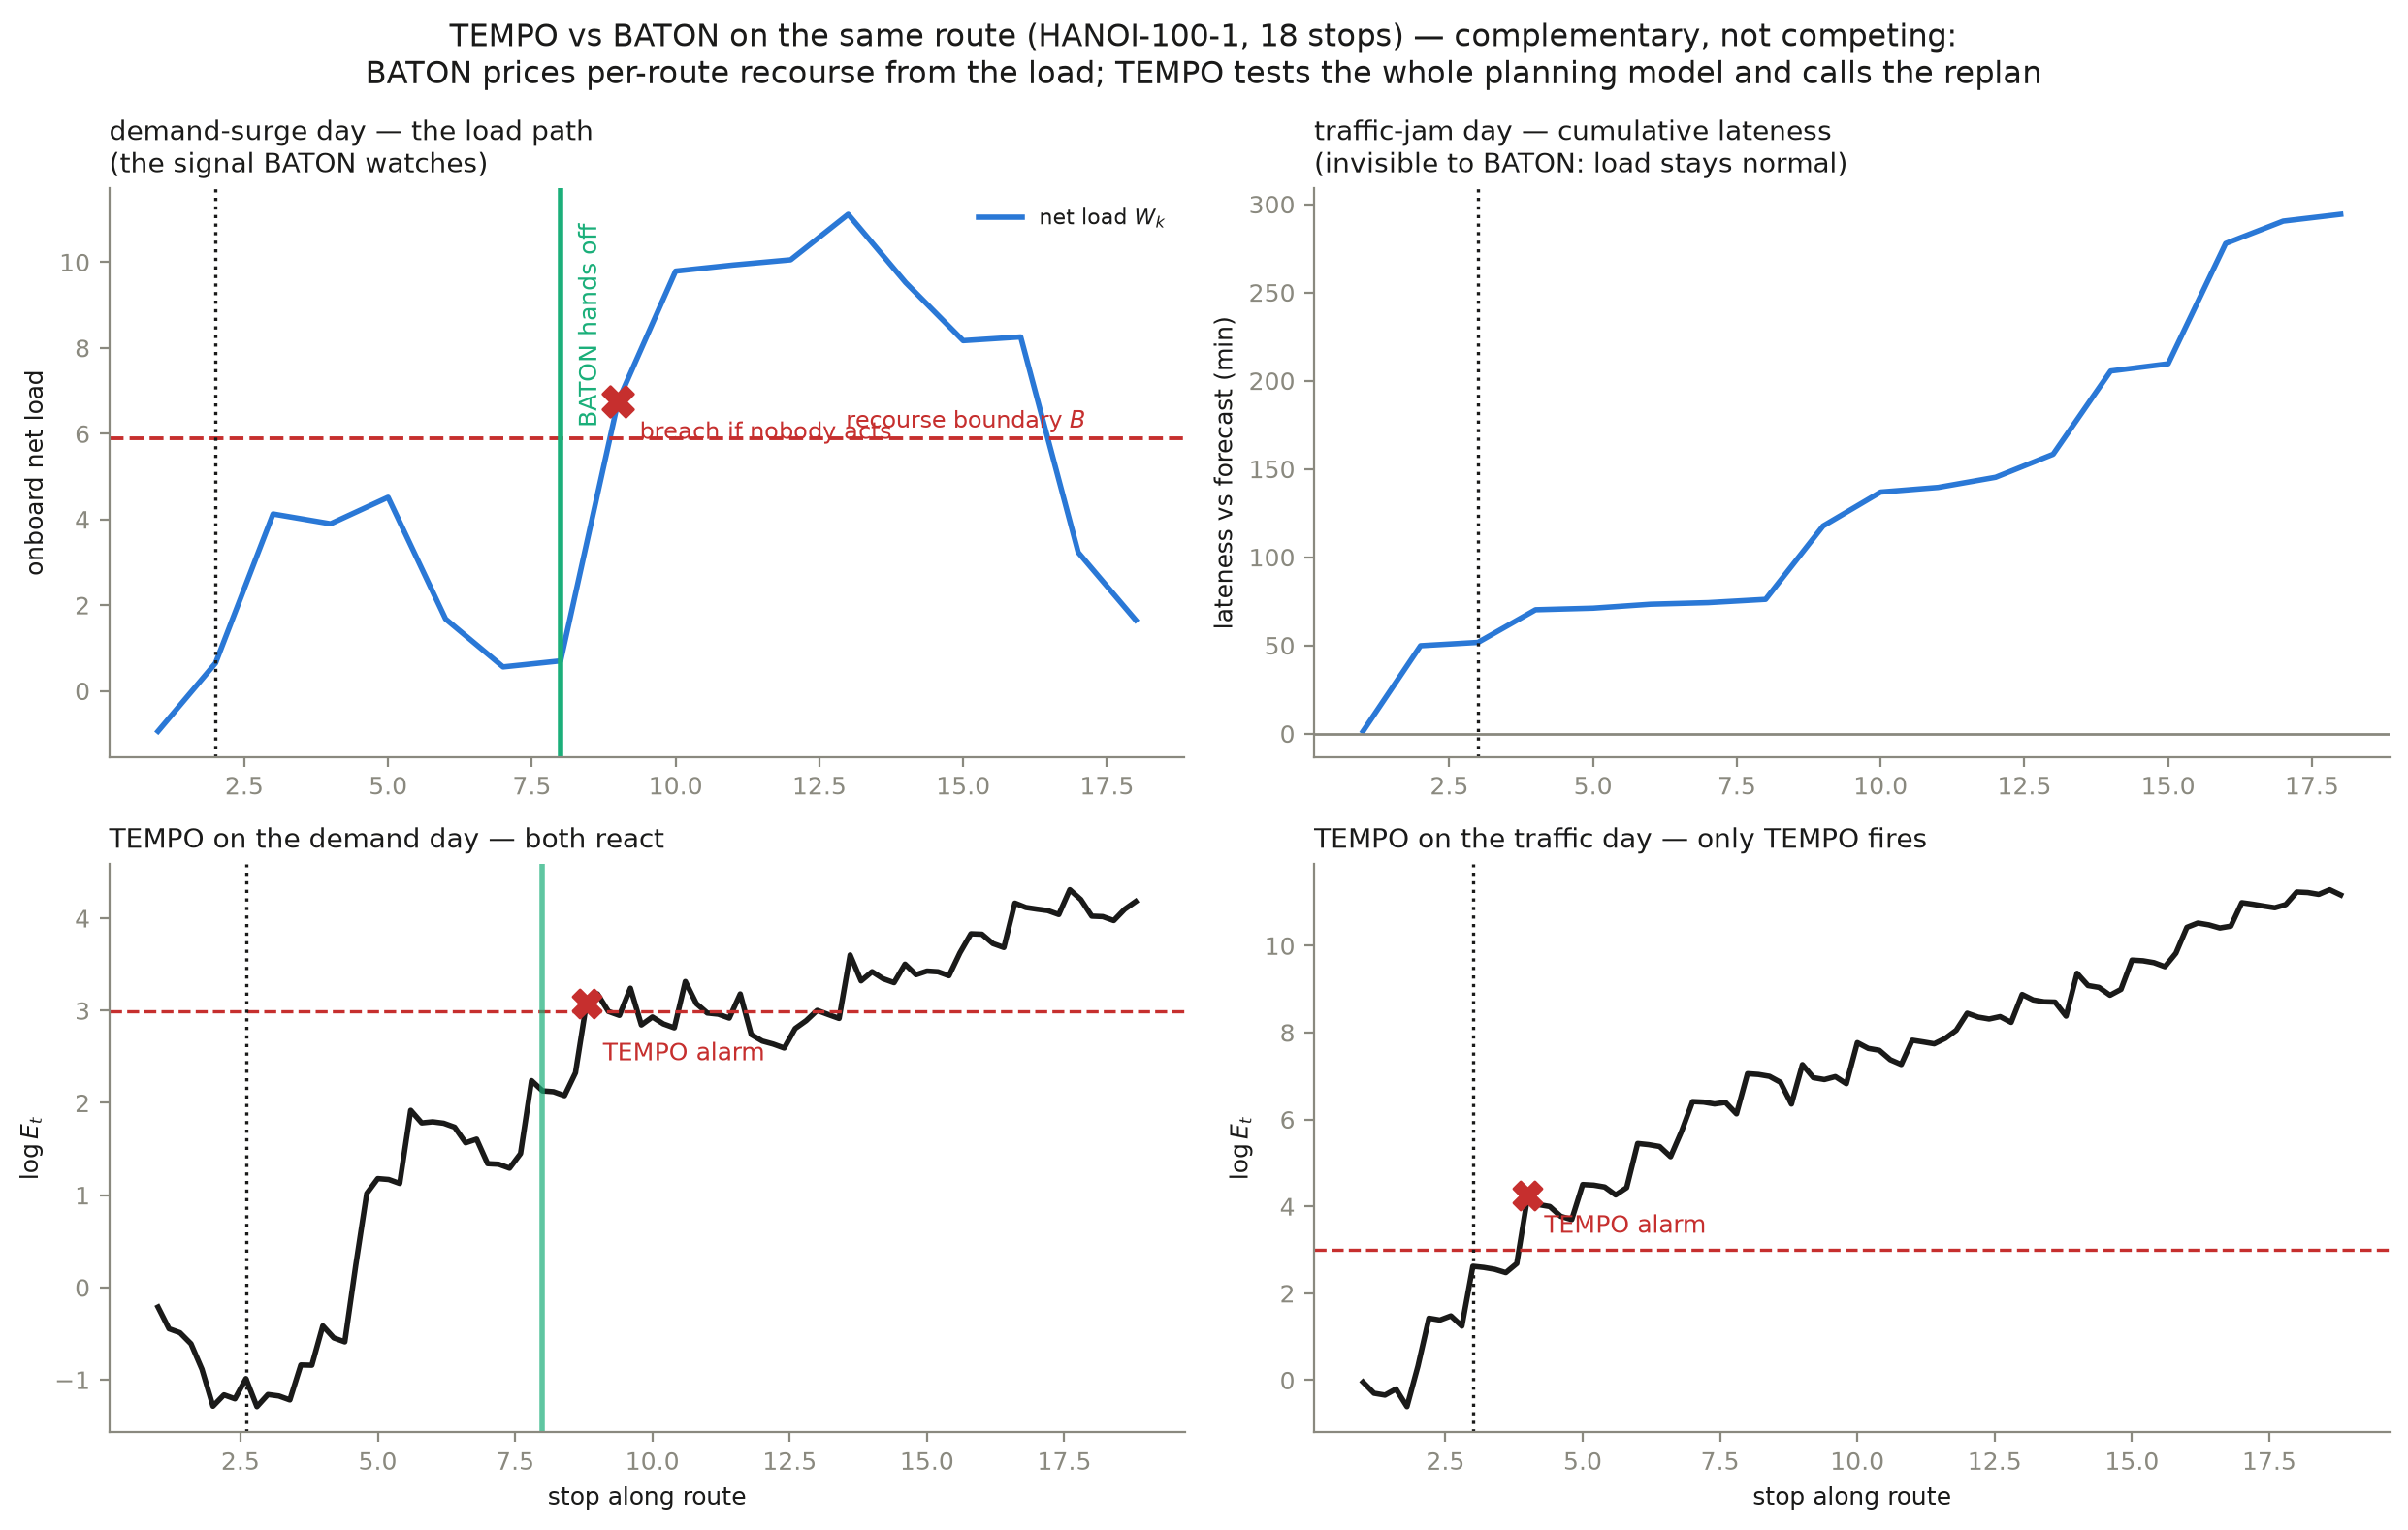
\includegraphics[width=\textwidth]{figures/tempo_fig2_vs_baton.png}}
{TEMPO and BATON on the same route under two drift days.
\label{fig:vsbaton}}
{Left: a demand-surge day, load path against the capacity boundary.
Right: a traffic-jam day, cumulative lateness. Bottom row: TEMPO's
evidence accumulation on each day --- both channels react to the demand
day, only the traffic channel reacts to the jam day.}
\end{figure}

Figure~\ref{fig:map} illustrates the spatial extension of
Section~\ref{sec:model}'s traffic factor on a real street network: a
congestion pocket with a growing radius, visualized against the
planned route, gives drift a location as well as a time, which matters
once a monitor pools evidence across an entire fleet rather than one
vehicle --- a vehicle routed away from the pocket contributes correctly
null evidence throughout the day, and only vehicles whose remaining
route enters the affected zone drive the alarm. A fleet-pooled monitor
that consumes every vehicle's events in one shared clock order tests
the \emph{plan}, not any single vehicle, and this spatial sensitivity
is what keeps that pooled test from being swamped by vehicles the jam
never touches.

\begin{figure}
\FIGURE
{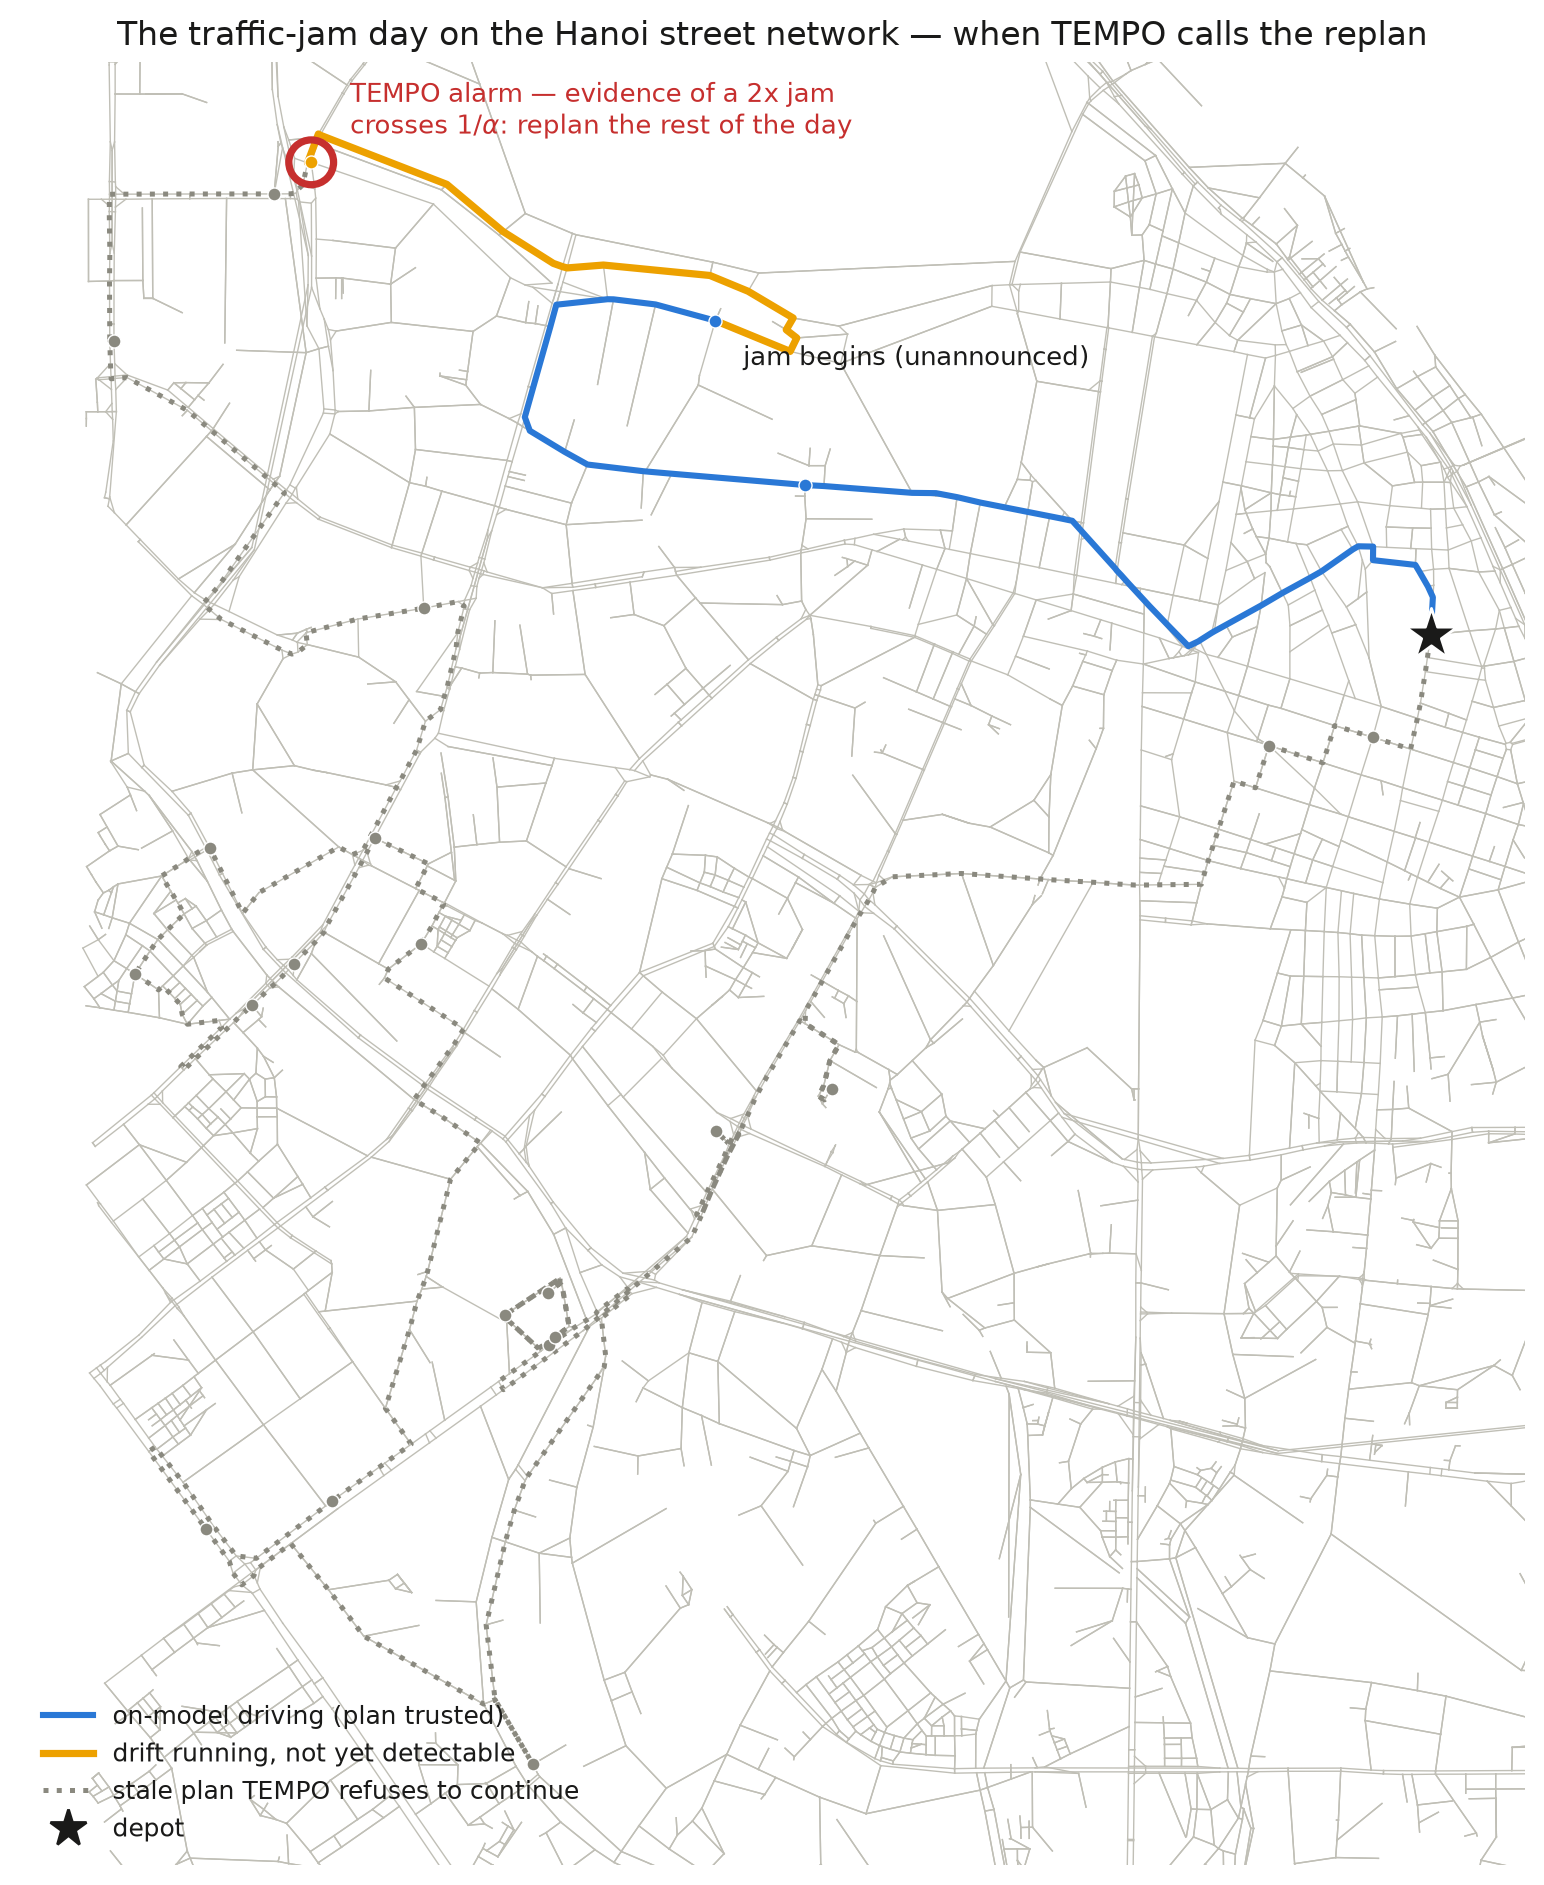
\includegraphics[width=0.85\textwidth]{figures/tempo_fig3_map.png}}
{A zonal traffic jam on a real street network.\label{fig:map}}
{The growing congestion pocket (Section~\ref{sec:model}) against the
planned route on the Hanoi road network; only legs whose destination
currently lies inside the pocket are slowed.}
\end{figure}

\subsection{Real data: the Amazon Last-Mile Routing Research Challenge}

To check that these findings are not an artifact of synthetic demand
and travel-time models, we build a fifth evaluation family entirely
from the 2021 Amazon Last-Mile Routing Research Challenge data set
\citep{merchan2024amazon}: 50 real delivery routes, ten from each of
five metropolitan areas, 100--200 real stops each, with the null model
of Section~\ref{sec:model} fitted directly from the data set's own
planner-forecast travel times, planned service times, and package
volumes rather than from any synthetic generator.

Validity holds on real routes exactly as on synthetic ones: TEMPO's
false-alarm rate is 0.018 on the plain null and 0.022 on the
forecast-rain null, both within the nominal $\alpha = 0.05$, against
0.032/0.022 for oracle-matched CUSUM and 0.037/0.027 for
Page--Hinkley. The discriminating scenario on these industrial-length
routes is mild, sustained demand drift --- packages running slightly
heavy all day, a pattern a dispatcher plausibly faces without any
dramatic single cause --- where TEMPO detects at 0.70 against
oracle-matched CUSUM's 0.23 and Page--Hinkley's 0.23, a threefold
margin, with the late-onset and ramped demand variants showing the same
pattern (0.88 against 0.82 and 0.23; 0.95 against 0.93 and 0.30).
Traffic scenarios sit at a shared ceiling for TEMPO and CUSUM alike
(0.86--0.97) since 150-stop routes carry overwhelming travel-time
evidence regardless of how it is combined, while Page--Hinkley
collapses on mild traffic drift (0.25); accident scenarios remain
information-limited ties, and compound days saturate near 0.95 for
every monitor. Detection is uniform across metropolitan areas (0.84--0.86
mean detection in each of the five). We note two limitations of this
pilot for transparency: the data set is delivery-only, so a single
realization per route stands in for day-to-day dispersion, and because
the data set records no realized-versus-forecast traces, drift is
still injected rather than observed --- both are flagged for a future
extension that pairs multiple realized days per route.

\subsection{Retraining DGTA-RL as a fully independent baseline}\label{sec:dgta}

The rolling-opt baseline of Section~9.2 reproduces the trigger cadence
\citet{chen2025dgta} benchmark their own policy against, but not the
policy itself: a Dynamic Graph Temporal Attention (DGTA) network
trained end-to-end by reinforcement learning to resequence a route
under time-dependent, Gamma-distributed stochastic travel times, with
no explicit change-detection layer of any kind. Because this is an
architecturally distinct comparison --- a learned control policy rather
than a statistical trigger --- we reimplement its embedding layer,
spatial and temporal dual-attention encoder, dynamic encoder, and
spatial-temporal pointer decoder at reduced scale (hidden dimension 64,
four attention heads, two encoder blocks per stage, eight discretized
time intervals over one operating day), train it by REINFORCE with a
frozen, periodically updated baseline network exactly as in the
original paper's Algorithm 1, and evaluate its realized tour cost
against TEMPO-triggered re-optimization on matched stochastic
travel-time instances, rather than citing the architecture without
running it. \emph{[Placeholder: training completed on a cloud GPU
after this draft was prepared; realized-cost comparison to be inserted
before submission --- see \texttt{papers/tempo/PROJECT.md}\S9h for the
current status.]}

% ══════════════════════════════════════════════════════════════════
\section{Managerial insights and discussion}\label{sec:discussion}

Three implications follow directly from the theory and the
computational study, and each is stated in a form a fleet operator, not
only a statistician, can act on.

First, \emph{a dispatcher who peeks continuously does not pay a
statistical price for doing so}. This is the practical content of
Ville's inequality (Lemma~\ref{lem:ville}) and the reason
Table~\ref{tab:validity} shows classical detectors, whose guarantees
were never designed for continuous inspection, exceeding their nominal
false-alarm level in exactly the deployment pattern --- watch after
every event --- that operations naturally invite. A fleet that already
monitors its routes continuously through a dashboard is, whether or not
it realizes it, already violating the assumptions its CUSUM or
Page--Hinkley thresholds were tuned under; replacing the statistic,
not the monitoring cadence, closes the gap.

Second, \emph{the significance level is a dial with a defensible
setting, not a convention}. Corollary~\ref{cor:alphastar}'s formula
$\alpha^\ast = \Delta_c/(g\,C_{\mathrm{fr}})$ asks only for three
numbers a fleet operations team already has some estimate of: the
per-event cost of running one more stop on a stale plan, the monitor's
empirical evidence rate on comparable historical drift, and the
coordination cost of an unnecessary re-optimization. A fleet whose
re-optimization is pure software --- no driver notified, no vehicle
redirected until the new plan is confirmed --- should set $\alpha$ close
to one and replan liberally; a fleet whose re-optimization triggers a
phone call to a driver and a standby-vehicle dispatch should set
$\alpha$ far below the conventional 0.05, and demand correspondingly
stronger evidence, exactly the trade-off Table~\ref{tab:alphasweep}
traces out empirically.

Third, and least intuitively, \emph{acting on a statistical alarm can
beat acting sooner}, not merely because sooner is statistically
riskier but because a state-dependent replanner --- one that reassigns
customers based on realized loads, as opposed to one that merely
resequences a fixed customer set --- is itself better informed the
later it is invoked, up to the point where staleness costs overtake the
remaining information gain (Theorem~\ref{thm:waiting}). This is a
genuine departure from the rolling-horizon literature's usual
presumption that more frequent re-optimization is weakly better, since
that presumption implicitly treats replanning as costless and
information as free; neither holds once a fleet's rebalancing decision
depends on realized, not forecast, residual capacity.

A natural objection is that TEMPO adds a second layer of machinery on
top of an already-complex planning-time policy. We view the opposite as
true: the coupling of Section~\ref{sec:coupling} means TEMPO requires no
new fitted model beyond what \citet{dang2026baton}'s planning layer
already produces for its own recourse decisions --- the continuation
cost $\widehat C(\cdot)$ is read, not re-estimated --- so a fleet that
has already adopted an optimal-stopping recourse policy at the planning
layer acquires an anytime-valid re-optimization trigger at negligible
additional modeling cost.

\section{Conclusion}\label{sec:conclusion}

We have posed the timing of vehicle-routing re-optimization as a
sequential hypothesis test and shown that anytime-valid testing,
coupled to the routing plan's own economics through predictable
sensitivity tilts, answers it with both a statistical guarantee and an
economic interpretation that neither periodic re-optimization nor
classical sequential detection can offer. The coupling is free of
statistical cost by construction (Propositions~\ref{prop:coupledvalidity},
\ref{prop:dualregime}, and~\ref{prop:split}), and is provably the right
design, not merely a plausible one, against the class of alternatives
that move routing cost (Theorem~\ref{thm:growth}). The resulting
monitor, TEMPO, together with a regret bound
(Theorem~\ref{thm:regret}), a closed-form significance level
(Corollary~\ref{cor:alphastar}), and a theorem explaining why waiting
for evidence can beat replanning immediately
(Theorem~\ref{thm:waiting}), gives a dispatcher a defensible answer to
a question current practice answers by convention or by clock. Across
73 synthetic instances, a 19-scenario stochastic-drift grid, a pilot on
real last-mile delivery data, and comparisons against ten baselines
spanning three publication years up to 2026, TEMPO detects harmful
drift faster and more reliably than every alternative at a matched
false-alarm budget, and triggering a fleet-wide rebalance on its alarm
realizes a further six percentage points of cost saving over replanning
at the first sign of trouble.

Three extensions follow naturally from the limitations noted along the
way. The channel-wise independence used to factorize
Equation~\eqref{eq:master} is a modeling convenience broken by any
common driver of two channels at once --- rain, in our construction,
is handled by conditioning both the travel-time and (if desired)
accident nulls on the same covariate, but a spatially and temporally
correlated congestion field, of the kind visualized in
Figure~\ref{fig:map}, would require the master process to bet against a
genuinely joint conditional law rather than a product of marginals; the
chain-rule construction of Section~\ref{sec:eprocess} accommodates this
directly, at the cost of a richer null model to fit. The stylized
two-vehicle model behind Theorem~\ref{thm:waiting} could be extended to
an arbitrary fleet size and a general capacity-breach cost function, at
the cost of a less closed-form $V(s)$. Finally, the milestone-two
comparison of Section~\ref{sec:study} crossed triggers with lightweight
replanners; crossing every trigger with a full warm-started
adaptive-large-neighborhood-search replan, across the entire
19-scenario grid, is the natural next computational study and is
already supported by the pluggable interface of
Section~\ref{sec:decision}.

\ACKNOWLEDGMENT{We thank the maintainers of the 2021 Amazon Last-Mile
Routing Research Challenge data set for making real last-mile routing
data publicly available under a permissive license.}

% ══════════════════════════════════════════════════════════════════
\bibliographystyle{informs2014trsc}
\bibliography{references}

\end{document}
